\documentclass[pdflatex,sn-mathphys-num]{sn-jnl}

\usepackage{graphicx}
\usepackage{multirow}
\usepackage{amsmath,amssymb,amsfonts}
\usepackage{amsthm}
\usepackage{mathrsfs}
\usepackage[title]{appendix}
\usepackage{booktabs}
\usepackage{url}

\theoremstyle{thmstyleone}
\newtheorem{theorem}{Theorem}
\newtheorem{proposition}[theorem]{Proposition}
\newtheorem{lemma}[theorem]{Lemma}
\newtheorem{corollary}[theorem]{Corollary}
\theoremstyle{thmstyletwo}
\newtheorem{remark}{Remark}
\theoremstyle{thmstylethree}
\newtheorem{definition}{Definition}

\raggedbottom

\begin{document}

\title[Finite-ensemble observability of the CBO mean-field rate]{Finite-ensemble observability of the mean-field convergence rate in consensus-based optimization}

\author*{\fnm{Rahul Kumar} \sur{Mishra}}\email{mishra.rahul98@gmail.com}

\affil*{\orgname{Independent Researcher}, \city{Ranchi}, \state{Jharkhand}, \country{India}}

\abstract{Consensus-based optimization (CBO) has a convergence guarantee for the implementable algorithm, assembled from a convergence result in mean-field law, a quantitative mean-field approximation and a discretization estimate. The guarantee is asymptotic in the ensemble size, and the constants carrying the parameter dependence sit in the prefactor rather than in the exponent. This paper asks a narrower question: which of those parameter dependencies are visible as effects on the slope fitted to a finite run, under experimental protocols that are stated and audited rather than assumed. Across $31\,320$ coupled realizations distributed over $2\,346$ cells of $12$ to $20$ realizations each, we report four results.

First, an inverse-temperature rule matched by objective spread produces an apparent dimension-dependent degradation of the fitted exponent of $0.96$ from $d=2$ to $d=40$. Calibrating the reference ensemble so that $\tau_{0,\infty}=\mathrm{ESS}_0(J_\infty)/J_\infty$ equals a target $\tau_0$, and fitting only over ensemble sizes $J\ge1/\tau_0$ at which that target is attainable, reduces it to $0.054$, $0.059$ and $0.078$ at $\tau_0=0.5$, $0.1$ and $0.01$. Both restrictions matter: a probe-calibrated fit over the full grid gives $0.030$, $0.099$ and $0.553$, and the formal dimension-concentration interaction that is resolved over the full grid, $+0.0305$ with interval $[+0.0123,+0.0479]$, is not resolved over the restricted one, $+0.0073$ with $[-0.0091,+0.0227]$.

Second, the remaining contrast is confounded and we report it as such. The nested subensembles whose error is measured are systematically further from their concentration target at $d=40$ than at $d=2$ at every size measured. A dedicated experiment that controls finite-ensemble concentration exactly, at the cost of one inverse temperature per ensemble size and therefore of changing the algorithm along the fitted $J$-curve, does not make the contrast vanish but is inconclusive about the mechanism of the residual.

Third, outside the parameter condition $2\lambda>d\sigma^2$ the onset is not resolvable from the boundary $r=d\sigma^2/(2\lambda)=1$, nine of ten bootstrap intervals containing it, while the severity is resolved: under the probe-calibrated protocol at nominal $\tau_0=0.1$, the non-admissible severity $\hat\gamma(3)-\hat\gamma(1)$ grows at $+0.144$ per doubling of $d$ with interval $[+0.123,+0.164]$ for isotropic diffusion and at $-0.002$ with $[-0.030,+0.027]$ for anisotropic. These experiments remain probe-calibrated at nominal $\tau_0=0.1$, and $r$ is shown to move the concentration trajectory itself, so the effect is not orthogonal to concentration.

Fourth, the parameter region in which the theorem applies and the region in which its exponent is visible in a finite run are different sets: admissible cells fail the operational criterion and non-admissible ones pass it. These finite-window results are not tests of, and do not contradict, the cited asymptotic convergence theorems; every quantity measured is a finite-window fitted slope and not an asymptotic rate.}

\keywords{consensus-based optimization, mean-field limit, propagation of chaos, effective sample size, derivative-free optimization}

\pacs[MSC Classification]{65K10, 90C56, 35Q84, 65C35}

\maketitle

\section{Introduction}\label{sec1}

Consensus-based optimization was introduced by Pinnau, Totzeck, Tse and Martin \cite{pinnau2017} and given an analytical framework by Carrillo, Choi, Totzeck and Tse \cite{carrillo2018}. Fornasier, Klock and Riedl \cite{fkr2024} proved convergence in mean-field law under mild assumptions and combined it with a quantitative mean-field approximation to obtain a convergence statement for the implementable scheme. Gerber, Hoffmann and Vaes \cite{ghv2025} removed the conditioning on a bounded event and obtained a pathwise mean-field limit at the classical Monte Carlo rate. Related lines include CBO on hypersurfaces \cite{fhps2020}, anisotropic variants for high-dimensional machine learning problems \cite{carrillo2021}, a compactness-based mean-field limit \cite{huangqiu2022}, constrained formulations \cite{borghi2023} and open implementations \cite{cbx2024}.

The quantitative theory has moved considerably since. Uniform-in-time mean-field estimates were obtained by Huang and Kouhkouh \cite{hk2025}, and by Bayraktar, Ekren and Zhou \cite{bez2026} in a weak sense on a bounded search domain. Gerber, Hoffmann, Kim and Vaes \cite{ghkv2025} proved uniform-in-time propagation of chaos with a prefactor depending explicitly on the problem parameters and report that for anisotropic noise this prefactor does not depend on the dimension. Ko\ss{}, Weissmann and Zech \cite{kwz2024} treat a class of consensus methods including CBO and CBS, and Beddrich, Chenchene, Fornasier, Huang and Wohlmuth \cite{beddrich2024} study the constrained problem and the practical few-particle regime.

Our question is therefore not whether the prefactor can be characterized theoretically. It increasingly can. It is which of the parameters governing it are visible in the fitted exponent of a finite run in the range of ensemble sizes studied here, and how much of the apparent dimension dependence survives once reference-ensemble initial concentration is controlled. Behaviour outside the stability condition has been examined before, including in \cite{beddrich2024}, and variants that alter the classical parameter restriction itself have been proposed, notably consensus-based optimisation with truncated noise \cite{frrs2025}. We claim no priority for studying $r>1$; the contribution here is the observability of the classical theory under the tested diffusion regime, not a study of stability thresholds in general. In the literature surveyed for this study we found no prior work that varies concentration systematically while holding the other experimental factors fixed and then evaluates the resulting dimension dependence of the fitted finite-ensemble exponent. The distinction from \cite{beddrich2024} is worth stating: that work studies how well CBO optimizes when the particle count is small, which is a question about the quality of the optimizer, whereas the question here is whether the proven mean-field rate is statistically visible in the fitted exponent of a run of that size, which is a question about what can be measured. The experiments below examine finite runs in which the benchmark rate may not be observable; they do not measure optimization quality, and no claim is made that the configurations studied here optimize well or badly.

There is a concrete version of the gap we address. Figure~1 of \cite{fkr2024} is produced on the Rastrigin objective at $\alpha=10^{15}$, $\lambda=1$, $\sigma=0.1$, $\Delta t=0.01$ with $N=32\,000$ agents in dimension two, and its Figure~2 at $\alpha=10^{15}$, $\lambda=1$, $\sigma=0.5$ with $N=320\,000$ in dimension one; the parameters are stated in the two captions. The experiment in \cite[Subsection 2.6]{ghv2025} verifies the $J^{-1}$ scaling of the squared coupled error at $\beta=3$, dimension two, with a reference ensemble of $10^6$ and $100$ realizations, and attributes small-$J$ breakdown to the effective sample size approaching one.

\subsection{What is and is not claimed}\label{sec:scope}

This paper does not measure the end-to-end guarantee of \cite[Theorem 3.8]{fkr2024}. The estimator is the coupled distance between a finite ensemble and a large reference ensemble, which addresses the mean-field approximation component and not the global optimization statement. The discretization step is held fixed at $\Delta t=0.01$ in both the finite ensemble and the reference, so that error is common-mode, largely cancels in the difference, and is not independently identified.

We do not claim any theorem is wrong. That the effective sample size matters at small $J$ is not new; it is observed in \cite[Subsection 2.6]{ghv2025}.

\subsection{Terminology and measured quantities}\label{sec:terms}

The $J^{-1}$ benchmark exponent for the squared coupled error is $-1$. Writing $\hat\gamma$ for the fitted slope of $\log\hat E$ against $\log J$ and $\Delta=-1-\hat\gamma$, a cell is \emph{rate-consistent at tolerance $0.15$} when the upper end of a bootstrap $95\%$ interval for $\hat\gamma$ is at most $-0.85$. A slope of $-0.85$ is not the proven rate; it is $15\%$ flatter in the exponent, and is nowhere described as recovery of the rate. Because $0.15$ is arbitrary, counts are reported at tolerances $0.10$, $0.15$ and $0.20$ throughout, and with Bonferroni-adjusted intervals.

Three concentration quantities appear and are never abbreviated to one symbol:
\[
\tau_0=\frac{\mathrm{ESS}_0}{J},\qquad
\bar\tau=\frac1T\int_0^T\frac{\mathrm{ESS}_t}{J}\,dt,\qquad
\tau_{\min}=\min_{t\le T}\frac{\mathrm{ESS}_t}{J}.
\]
Experiments control $\tau_0$. Section~\ref{sec:sigma} finds $\bar\tau/\tau_0$ between $0.003$ and $4.0$.

\emph{Grids and the estimator.} The ensemble sizes are $J\in\{10,20,40,80,160,320,640,1280,2560,5000\}$, with the reference at $J_\infty=5\times10^4$ so that no $J$ exceeds $J_\infty/10$; the reference-size arm uses $J_\infty\in\{12\,500,25\,000,50\,000,100\,000\}$ on the common grid capped at $J\le1250$. The horizon is $T=1$ with $\Delta t=0.01$, so $K=100$ steps, and the supremum over $t\in[0,T]$ in the error is realized as a maximum over the $K+1$ grid points; we write it as a supremum only for notational continuity with the cited bounds. The estimator averages the per-particle maximum of the \emph{squared} distance, matching the form in which the mean-field bounds are stated: it is $\frac1M\sum_m\frac1J\sum_j\max_k\|\cdot\|^2$ as written in \eqref{eq:est}, not an estimate of $\sup_t\mathbb E[\|\cdot\|^2]$ or of $\sup_t\frac1J\sum_j\|\cdot\|^2$. The square is not cosmetic: fitting the unsquared distance would halve every exponent reported here. The three orderings are different functionals and the one measured here is deliberately the first, because it is the quantity evaluated by the experimental protocol in a single coupled simulation; comparisons with bounds stated for a different ordering are therefore qualitative, and we do not treat agreement or disagreement with them as a test.

Two concentration quantities are distinguished throughout and the distinction is the conceptual heart of Sections~\ref{sec:calib} and \ref{sec:finitej}: $\tau_{0,\infty}=\mathrm{ESS}_0(J_\infty)/J_\infty$ is the initial concentration of the reference ensemble, and $\tau_{0,J}=\mathrm{ESS}_0(J)/J$ is that of the finite ensemble of size $J$ whose error is measured. Setting $\tau_{0,\infty}=\tau_0$ does not set $\tau_{0,J}=\tau_0$, and Section~\ref{sec:finitej} shows the gap between them varies systematically with dimension. Population concentration is represented by $1/\varrho_\beta$ with $\varrho_\beta=\mathbb E[w^2]/\mathbb E[w]^2$; the empirical effective sample size fraction estimates it and is asymptotically equal to it. Statements about $\tau$ below are empirical unless $\varrho_\beta$ is written explicitly. The \emph{typical slope-SE scale}, referred to below as the noise floor for brevity, is defined as the median over cells of the standard error of $\hat\gamma$. Two estimators are available and they do not agree. The delta method propagated from per-$J$ standard errors treats the ten $J$ values as independent, which they are not: one coupled realization contributes to every $J$, so the per-$J$ errors are positively correlated and the propagated standard error is biased downward. Over the $1\,344$ cells with per-$J$ errors archived it gives $0.0219$ with interquartile range $[0.0163,0.0291]$. The realization-level bootstrap respects the dependence, since all $J$ values within a realization move together and the slope is refitted on each resample; over the $420$ cells with per-realization slopes archived it gives a median of $0.0260$ with interquartile range $[0.0191,0.0341]$, about nineteen percent larger. We use $0.0260$, referred to as the bootstrap slope-SE reference scale, as the yardstick wherever a comparison is made, note that the two populations of cells are not the same, and treat both as descriptive scales rather than confidence bounds. Over the $1\,344$ cells with stored intervals it is $0.0219$, interquartile range $[0.0163,0.0291]$. Effects are compared against this value and never against an undefined one.

Finally, $r$ denotes the dimensionless diffusion-to-drift parameter ratio of \cite[Theorem 3.7]{fkr2024}:
\[
r_{\rm iso}=\frac{d\sigma^2}{2\lambda},\qquad r_{\rm aniso}=\frac{\sigma^2}{2\lambda},
\]
so $r=1$ is the boundary in each case.

\section{Setting}\label{sec2}

We use CBO in the form of the Euler--Maruyama scheme of \cite{fkr2024}, drift parameter $\lambda$, diffusion parameter $\sigma$, inverse temperature $\alpha$, consensus point the Boltzmann-weighted mean with weights $\exp(-\alpha\mathcal E(v))$. For mean-field results we follow \cite{ghv2025}: inverse temperature $\beta$, ensemble size $J$. Both diffusion types are used and are written explicitly, since Section~\ref{sec:aniso} compares them:
\begin{align}
\text{isotropic:}\quad & dX=-\lambda\,(X-v)\,dt+\sigma\,\|X-v\|_2\,dB,\label{eq:iso}\\
\text{anisotropic:}\quad & dX=-\lambda\,(X-v)\,dt+\sigma\,\mathrm{diag}(X-v)\,dB.\label{eq:aniso}
\end{align}

\begin{definition}[{\cite[Assumption H]{ghv2025}}]\label{def:AH}
A function $f:\mathbb R^d\to\mathbb R$ bounded below by $f_\star$ lies in $\mathcal A(s,\ell,u)$ when
\begin{align}
|f(x)-f(y)|&\le L_f(1+|x|+|y|)^s|x-y|,\label{eq:G1}\\
f(x)-f_\star&\le c_u|x|^u+C_u,\label{eq:G2a}\\
f(x)-f_\star&\ge c_\ell|x|^\ell-C_\ell,\label{eq:G2b}
\end{align}
with $u\ge\ell\ge0$. The main results of \cite{ghv2025} require $\ell=u$.
\end{definition}

\cite[Theorem 3.7]{fkr2024} is stated for a weak solution of the mean-field Fokker--Planck equation that is assumed to exist, and does not itself impose growth conditions; the only existence result supplied for it is \cite[Theorem 3.2]{fkr2024}, whose hypothesis requires
\begin{align}
|\mathcal E(v)-\mathcal E(w)|&\le C_1(\|v\|_2+\|w\|_2)\|v-w\|_2,\label{eq:F19}\\
\mathcal E(v)-\underline{\mathcal E}&\le C_2(1+\|v\|_2^2),\label{eq:F20}
\end{align}
and either $\sup\mathcal E<\infty$ or $\mathcal E(v)-\underline{\mathcal E}\ge C_3\|v\|_2^2$ for $\|v\|_2\ge C_4$. Condition \eqref{eq:F19} is \eqref{eq:G1} with $s=1$ and no additive constant, so the hypothesis of \cite{fkr2024} is strictly narrower than the class of \cite{ghv2025}.

\section{The assumption audit}\label{sec3}

The purpose of this section is to establish that the objectives used below span materially different regularity classes.

\begin{table}[h]
\caption{Classification of seven standard benchmarks.}\label{tab:class}
\begin{tabular}{@{}p{2.6cm}p{2.9cm}ccp{3.1cm}@{}}
\toprule
Objective & Class & \eqref{eq:F19} & \eqref{eq:F20} & \cite{ghv2025} main results\\
\midrule
Sphere & $\mathcal A(1,2,2)$ & yes & yes & covered\\
Rastrigin & $\mathcal A(1,2,2)$ & yes & yes & covered\\
Griewank & $\mathcal A(1,2,2)$ & yes & yes & covered\\
Ackley & $\mathcal A(0,0,0)$ & yes & yes & covered\\
Levy & $\mathcal A(2,2,2)$ & no & yes & covered\\
Rosenbrock & $\mathcal A(3,1,4)$ & no & no & \textbf{no}, $\ell\ne u$\\
Schwefel on $\mathbb R^d$ & unbounded below, in no class & --- & --- & theorem does not apply\\
Schwefel on $[-500,500]^d$ & bounded and Lipschitz & yes & yes & $\mathcal A$ is defined on $\mathbb R^d$ and is not applied here\\
\botrule
\end{tabular}
\end{table}

\subsection{Levy fails \eqref{eq:F19}}\label{sec:levy}

\begin{proposition}
Levy's function lies in $\mathcal A(2,2,2)$ and not in $\mathcal A(1,\cdot,\cdot)$, hence fails \eqref{eq:F19}.
\end{proposition}

\begin{proof}
With $w_i=1+(x_i-1)/4$, consider the summand $g(w)=(w-1)^2(1+10\sin^2(\pi w+1))$. Then
\[
g'(w)=2(w-1)\bigl(1+10\sin^2(\pi w+1)\bigr)+20\pi (w-1)^2\sin(\pi w+1)\cos(\pi w+1).
\]
The first term is bounded by $22|w-1|$. The second is bounded by $10\pi(w-1)^2$ and attained: at $w$ with $\sin(\pi w+1)\cos(\pi w+1)=1/2$ one has $|g'(w)|\ge 10\pi(w-1)^2-22|w-1|$, which grows quadratically. Hence $\sup|\nabla f|$ grows like $|x|^2$, and the mean value theorem gives \eqref{eq:G1} with $s=2$, attained. Condition \eqref{eq:F19} requires exponent $1$. Growth is quadratic above and below after the affine change of variable.
\end{proof}

\subsection{Rosenbrock}\label{sec:rosen}

\begin{proposition}\label{prop:rosen}
Rosenbrock's function lies in $\mathcal A(3,1,4)$, with $c_\ell=1/(8\sqrt d)$ and $C_\ell=1$. Conditions \eqref{eq:F19} and \eqref{eq:F20} fail.
\end{proposition}

\begin{proof}
Write $f(x)=\sum_{i=1}^{d-1}\bigl[100(x_{i+1}-x_i^2)^2+(1-x_i)^2\bigr]$, $f_\star=0$ at the all-ones point.

\emph{$u=4$.} Each term is at most $100(|x_{i+1}|+x_i^2)^2+(1+|x_i|)^2\le C(1+|x|^4)$; the exponent is attained along $x_{i+1}=0$, $x_i=t$, where $f\ge100t^4$.

\emph{$s=3$.} $\partial f/\partial x_i$ contains $-400x_i(x_{i+1}-x_i^2)$, which grows like $|x|^3$ and dominates; the mean value theorem gives \eqref{eq:G1} with $s=3$ and no smaller.

\emph{$\ell\le1$.} On the curve $x_i=t^{2^{i-1}}$, $t>1$, every coupling term vanishes and $f=\sum_{i=1}^{d-1}(1-x_i)^2$. The norm is dominated by the last coordinate, $|x|\asymp t^{2^{d-1}}$, and the largest term of $f$ is $(1-t^{2^{d-2}})^2\asymp t^{2^{d-1}}\asymp|x|$. So $f$ grows linearly in $|x|$ along this curve and no bound $f\ge c|x|^\ell-C$ can hold with $\ell>1$.

\emph{$\ell\ge1$.} We show $f(x)\ge|x|/(8\sqrt d)-1$ for every $x\in\mathbb R^d$, $d\ge2$. Put $M=\max_i|x_i|$, so that $M\le|x|\le\sqrt d\,M$. If $M<8$ then $|x|/(8\sqrt d)\le1$ and the bound is immediate from $f\ge0$, so assume $M\ge8$ and let $k$ attain the maximum. It suffices to prove $f(x)\ge M/8$.

\emph{Case $k=1$.} The summand $i=1$ contains $(1-x_1)^2\ge(M-1)^2$, and $(M-1)^2\ge M/8$ for $M\ge2$.

\emph{Case $k\ge2$.} Consider the summand $i=k-1$, which is present because $2\le k\le d$. Write $a=x_{k-1}$.

If $|x_k-a^2|\ge\sqrt M/20$, then $100(x_k-a^2)^2\ge100\cdot M/400=M/4\ge M/8$.

Otherwise $|x_k-a^2|<\sqrt M/20$. Since $a^2\ge0$, if $x_k=-M$ then $|x_k-a^2|=M+a^2\ge M>\sqrt M/20$ for $M\ge1$, a contradiction; hence $x_k=M$. Then $a^2>M-\sqrt M/20\ge M(1-1/20)=0.95M$, using $\sqrt M\le M$ for $M\ge1$, so $|a|>\sqrt{0.95M}$. For either sign of $a$ one has $(1-a)^2\ge(|a|-1)^2$, and $\sqrt{0.95M}\ge2$ once $M\ge4.22$, so
\[
(1-a)^2\ \ge\ \bigl(\sqrt{0.95M}-1\bigr)^2\ \ge\ \Bigl(\tfrac12\sqrt{0.95M}\Bigr)^2\ =\ 0.2375\,M\ \ge\ M/8 .
\]
In every case $f(x)\ge M/8\ge|x|/(8\sqrt d)$, which is \eqref{eq:G2b} with $\ell=1$.

\emph{Failure of \eqref{eq:F19}, \eqref{eq:F20}.} The gradient grows like $|x|^3$ and $f$ like $|x|^4$.
\end{proof}

\begin{remark}\label{rem:rosen}
The constant $c_\ell=1/(8\sqrt d)$ degrades with the dimension. Definition~\ref{def:AH} permits constants depending on the function, and hence on $d$, but the degradation is worth recording: the lower growth is linear in $|x|$ for every $d$, with a coefficient that shrinks like $d^{-1/2}$.

The numerical evidence below is a consistency check and not part of the proof. The sphere search returns an \emph{upper} bound on $m(R)=\min_{|x|=R}f(x)$, so it can corroborate $m(R)\lesssim R$ and not $m(R)\gtrsim R$; the latter is supplied by the argument above.
\end{remark}

Minimizing $f$ on spheres of radius $R$, starting a projected local search from the curve with its parameter fixed by bisection, gives fitted exponents $1.0500$, $1.0417$, $1.0409$, $1.0423$ at $d=2,3,5,10$, and $m(10^6)=998\,000$, $998\,938$, $998\,962$, $998\,962$. An earlier run without the curve-parameterized start returned $1.4157$ at $d=5$ with numerical-differentiation overflow warnings and was treated as a solver failure.

\subsection{Schwefel}\label{sec:schwefel}

\begin{proposition}
$f(x)=418.9829\,d-\sum_i x_i\sin\sqrt{|x_i|}$ is unbounded below on $\mathbb R^d$, hence lies in no $\mathcal A(s,\ell,u)$; on $[-500,500]^d$ it is bounded and Lipschitz.
\end{proposition}

\begin{proof}
Take $x_i=(\pi/2+2k\pi)^2$, so $\sin\sqrt{x_i}=1$ exactly and $f=418.9829\,d-d(\pi/2+2k\pi)^2\to-\infty$. On the box, $f$ is continuous on a compact set, and $\frac{d}{dx}[x\sin\sqrt x]=\sin\sqrt x+\frac{\sqrt x}2\cos\sqrt x$ is bounded there.
\end{proof}

At $k=500$: $x_i=9.879\times10^6$, $\|x\|=2.209\times10^7$, $f=-4.940\times10^7$ at $d=5$; the fitted slope of $\log(-f)$ against $\log\|x\|$ is $1.0440$. On the box the minimum is $0.000013$ at $x_i=420.9685$ and the maximum $837.97$. The box classification concerns a restricted domain and is not covered by the unconstrained theorem; the constrained problem is analysed in \cite{borghi2023,beddrich2024}.

\subsection{Two branches, three independent sources}\label{sec:branches}

Bounded and coercive objectives are treated differently at three separate points. \cite[Lemma 3.3]{carrillo2018} bounds the second moment of the weighted mean by $b_1+b_2\int|x|^2d\rho$ with $b_2$ decreasing in $\alpha$ for coercive $f$, and \cite[Remark 3.1]{carrillo2018} states the estimate does not blow up as $\alpha\to\infty$. For bounded $f$ the corresponding bound carries $\exp(\alpha(\sup f-\inf f))$, and \cite[Remark 4.1]{carrillo2018} observes it diverges. the moment condition of \cite[Assumption H]{ghv2025} requires $p_{\mathcal M}=s+2$ when $\ell=0$ against $1$ when $\ell>0$. The same split is carried forward into the chain traced in Supplementary Material~S1: the proof of \cite[Lemma 3.10]{fkr2024} records $b_1=0$ and $b_2=\exp(\alpha(\sup\mathcal E-\underline{\mathcal E}))$ for bounded $\mathcal E$, against $b_1=C_4^2+b_2$ and $b_2=2(C_2/C_3)(1+1/(\alpha C_3C_4^2))$, decreasing in $\alpha$, for coercive $\mathcal E$. Ackley is on the unfavourable side of all four.

\section{Constant tracing}\label{sec4}

These observations concern bookkeeping in published upper bounds. None is a claim about the behaviour of CBO, none is used in Section~\ref{sec7}, and the chain is in Supplementary Material~S1.

\emph{A parameter condition that is also a scaling constraint.} The constant
\[
c(\vartheta,\lambda,\sigma)=\min\Bigl\{\tfrac{\vartheta}{2}\tfrac{2\lambda-d\sigma^2}{\sqrt2(\lambda+d\sigma^2)},\ \sqrt{\vartheta\tfrac{2\lambda-d\sigma^2}{d\sigma^2}}\Bigr\}
\]
introduced in the proof of \cite[Theorem 3.7]{fkr2024} vanishes as $d\sigma^2\uparrow2\lambda$. Near that boundary the first argument is linear in $2\lambda-d\sigma^2$ and the second is of square-root order, so the minimum is attained at the first and $c\asymp2\lambda-d\sigma^2$. The leading factor of the informal lower bound on $\alpha_0$ derived in \cite[Remark 4.8]{fkr2024} is $c^{-2}$, and the logarithm it multiplies also diverges as $c\downarrow0$, so $\alpha_0$ grows at least like $(2\lambda-d\sigma^2)^{-2}$ near the boundary and a dimension-uniform reading requires $\sigma=O(d^{-1/2})$. Sections~\ref{sec:sigma}--\ref{sec:onset} measure this axis.

\emph{Nested worst-case $\alpha$-dependence.} Tracing the constants in the proofs of \cite[Lemma 3.10 and Proposition 3.11]{fkr2024} gives a mean-field constant whose published chain is exponential in $\alpha$ inside a Gr\"onwall exponentiation, with a second such channel that is present for bounded objectives and absent for coercive ones (Supplementary Material~S1). This is propagation of worst cases; the composition of upper bounds says nothing about the true constant, and \cite[Theorem 3.8]{fkr2024} itself claims only exponential dependence on $\alpha$.

\emph{A complexity coupling.} \cite[Remark 3.9]{fkr2024} states the cost as $O(KN)$; \cite[Theorem 3.8]{fkr2024} states $C_{\rm NA}$ depends linearly on $N$. With $m=1/2$, $\Delta t\lesssim1/N$ and $K\gtrsim N$, so the stated sufficient conditions imply a requirement of at least order $N^2$. This is a lower bound on the requirement, $\Omega(N^2)$, not an upper bound on runtime; no matching upper bound is established and no runtime was measured.

\section{A finite-sample bound in terms of the effective sample size}\label{sec5}

The weighted mean is a self-normalized importance-sampling estimator, a class studied in \cite{agapiou2017} and whose ratio moments are treated in \cite{doukhan2009}; \cite{ghv2025} routes its own Lemma 3.7 through the latter. That lemma bounds $\mathbb E|\mathcal M_\beta(\mu^J)-\mathcal M_\beta(\mu)|^p\le CJ^{-p/2}$ with $C$ depending on $(f,\beta,p,r)$ and the $r$-th moment of $\mu$, the concentration being absorbed into $C$. The bound below is a direct finite-sample specialization that keeps the concentration ratio visible instead. We do not claim the inequality itself is new; its role here is to name the quantity that the experiments control.

\begin{theorem}\label{thm:ess}
Let $X^1,\dots,X^J$ be i.i.d.\ from $\rho\in\mathcal P(\mathbb R^d)$, let $w=e^{-\beta f}$ with $f$ bounded below, and assume $\rho[w^2]<\infty$ and $\rho[w^2|x-M|^2]<\infty$, where $M=\mathcal M_\beta(\rho)$. Put $\hat N=\frac1J\sum_j w(X^j)X^j$, $\hat D=\frac1J\sum_j w(X^j)$, $\hat M=\hat N/\hat D$,
\[
\varrho_\beta=\frac{\rho[w^2]}{\rho[w]^2},\qquad \eta_2=\frac{w^2\rho}{\rho[w^2]},\qquad s^2=\eta_2\bigl[|x-M|^2\bigr],
\]
and $A_J=\{\hat D\ge\rho[w]/2\}$. Then
\begin{equation}\label{eq:thm}
\mathbb P(A_J^c)\le\frac{4(\varrho_\beta-1)}{J},\qquad
\mathbb E\bigl[|\hat M-M|^2\mathbf1_{A_J}\bigr]\le\frac{4\varrho_\beta s^2}{J},
\end{equation}
and $\hat\tau_J=(\sum_jw_j)^2/(J\sum_jw_j^2)\to1/\varrho_\beta$ almost surely.
\end{theorem}

\begin{proof}
\emph{Step 1.} Put $Z_j=w(X^j)(X^j-M)$. By definition of $M$, $\mathbb E[Z]=\rho[wx]-M\rho[w]=0$.

\emph{Step 2.} $\hat N-M\hat D=\frac1J\sum_jZ_j$ identically, so $\hat M-M=\bigl(\frac1J\sum_jZ_j\bigr)/\hat D$.

\emph{Step 3.} On $A_J$, $|\hat M-M|\le\frac2{\rho[w]}\bigl|\frac1J\sum_jZ_j\bigr|$.

\emph{Step 4.} The $Z_j$ are i.i.d.\ with mean zero, so $\mathbb E\bigl|\frac1J\sum_jZ_j\bigr|^2=\frac1J\rho[w^2|x-M|^2]$.

\emph{Step 5.} Combining and factoring,
\[
\mathbb E\bigl[|\hat M-M|^2\mathbf1_{A_J}\bigr]\le\frac{4}{\rho[w]^2}\cdot\frac{\rho[w^2|x-M|^2]}{J}
=\frac4J\cdot\frac{\rho[w^2]}{\rho[w]^2}\cdot\frac{\rho[w^2|x-M|^2]}{\rho[w^2]}=\frac{4\varrho_\beta s^2}{J}.
\]

\emph{Step 6.} $\operatorname{Var}(\hat D)=\frac1J(\rho[w^2]-\rho[w]^2)$, so Chebyshev at deviation $\rho[w]/2$ gives the first bound.

\emph{Step 7.} $\hat\tau_J\to\rho[w]^2/\rho[w^2]$ almost surely by the strong law, and $\varrho_\beta\ge1$ by Cauchy--Schwarz.
\end{proof}

\begin{corollary}\label{cor:tauJ}
With $\tau=1/\varrho_\beta$, $\mathbb E[|\hat M-M|^2\mathbf1_{A_J}]\le4s^2/(\tau J)$ and $\mathbb P(A_J^c)\le4/(\tau J)$: concentration enters the prefactor and not the exponent, and the discarded-event bound is non-vacuous only for $J>4(1/\tau-1)$.
\end{corollary}

\begin{remark}[scope]\label{rem:thmscope}
Theorem~\ref{thm:ess} concerns i.i.d.\ samples and corresponds to \cite[Lemma 3.7]{ghv2025}, one of three terms in Sznitman's argument; the full mean-field constant also carries a Wasserstein stability estimate and a Gr\"onwall factor. It does not predict that the fitted slope of the full interacting system bends at any particular $J$. Section~\ref{sec:thmcheck} reports an empirical consistency check motivated by the bound, not a verification of it. The Chebyshev step is crude: at $\tau=0.1$ the bound is vacuous below $J=36$, while the measured exponent is $-1.02$ from $J=10$ upward.
\end{remark}

\begin{lemma}\label{lem:sat}
For normalized weights, $\mathrm{ESS}=(\sum_iw_i^2)^{-1}$ satisfies $1/w_{\max}\le\mathrm{ESS}\le1/w_{\max}^2$, and $\mathrm{ESS}=1$ if and only if some $w_i=1$. For Boltzmann weights at finite $\beta$ and finite objective values every $w_i$ is strictly positive, so that case is approached and not attained in exact arithmetic; it occurs in an implementation when the subdominant weights underflow, which is the saturated case treated in the corollary below. Moreover $\beta\mapsto\log\mathrm{ESS}(\beta)$ is non-increasing.
\end{lemma}

\begin{proof}
$\sum_iw_i^2\le w_{\max}\sum_iw_i=w_{\max}$ gives $\mathrm{ESS}\ge1/w_{\max}$; $\sum_iw_i^2\ge w_{\max}^2$ gives the upper bound. Since $\sum_iw_i^2\le\sum_iw_i=1$ with equality if and only if every $w_i\in\{0,1\}$, $\mathrm{ESS}=1$ exactly when one weight is $1$. For monotonicity, with $S_k(\beta)=\sum_ie^{-k\beta f_i}$ one has $\log\mathrm{ESS}=2\log S_1-\log S_2$ and
\[
\frac{d}{d\beta}\log\mathrm{ESS}=-2\,\mathbb E_\beta[f]+2\,\mathbb E_{2\beta}[f]\le0,
\]
where $\mathbb E_{k\beta}$ is expectation under weights proportional to $e^{-k\beta f}$ and $\partial_k\mathbb E_{k\beta}[f]=-\beta\operatorname{Var}_{k\beta}(f)\le0$.
\end{proof}

\begin{corollary}\label{cor:notartifact}
Ordering $f(x_{(1)})\le f(x_{(2)})\le\cdots$,
\[
\|v_\alpha-x_{(1)}\|\le\Bigl(\sum_{i\ge2}e^{-\beta(f_i-f_1)}\Bigr)\max_i\|x_i-x_{(1)}\|.
\]
When the suboptimal shifted weights underflow, the implemented weights are numerically saturated. Whether the computed consensus differs materially from the exact weighted mean is controlled by this tail sum, which involves the particle count and the cloud diameter and not only the second-smallest objective gap. The underlying weight concentration persists independently of the floating-point format, although the value of $\beta$ at which saturation occurs depends on the precision.
\end{corollary}

\section{Experimental method}\label{sec6}

We follow \cite[Subsection 2.6]{ghv2025} in structure. A reference ensemble of $J_\infty$ particles is evolved; for each smaller $J$ an ensemble of $J$ particles is started from the same initial positions and driven by the same Brownian increments as the reference ensemble's first $J$ particles, each computing its own consensus point. Because the drift depends on the empirical consensus, the trajectories differ even under common noise, and that difference is measured:
\begin{equation}\label{eq:est}
\hat E_{J,J_\infty}=\frac1{MJ}\sum_{m=1}^M\sum_{j=1}^J\sup_{t\in[0,T]}\bigl\|X^{(j/J,m)}_t-X^{(j/J_\infty,m)}_t\bigr\|^2 .
\end{equation}
The subscript is retained because the reference is a proxy and not the mean-field limit.

Parameters follow \cite[Table 1]{ghv2025} where possible: $\Delta t=0.01$, $T=1$, $\lambda=1$, and $\sigma=1/5$ except where $\sigma$ is swept. Two deviations are forced by hardware: $J_\infty=5\times10^4$ rather than $10^6$, and $12$ to $20$ realizations rather than $100$. No $J$ above $J_\infty/10$ is reported.

\emph{Objectives.} Six named benchmarks, plus a synthetic family
\begin{equation}\label{eq:synth}
f_{\kappa,\rho,\omega}(x)=\sum_{i=1}^d a_i x_i^2+\rho\sum_{i=1}^d\bigl(1-\cos(\omega x_i)\bigr),
\qquad a_i=\kappa^{(i-1)/(d-1)},
\end{equation}
with global minimum $0$ at the origin for all parameter values, so that $\kappa$ is the condition number of the quadratic part, $\rho$ the modality amplitude and $\omega$ the ruggedness frequency. Each generating parameter can be varied without moving the others, but they are not geometrically independent: the second derivative of the cosine term is $\rho\omega^2\cos(\omega x)$, so changing $\omega$ at fixed $\rho$ also changes local curvature. When these parameters are used as predictors in Section~\ref{sec:law} they are nominal generator settings, not independent geometric factors. Section~\ref{sec:suff} uses $\kappa\in\{1,100\}$, $\rho\in\{0,5,20\}$, $\omega\in\{1,3\}$; Section~\ref{sec:law} uses $\omega\in\{1,3,7\}$ with a single $\omega$ level at $\rho=0$, where $\omega$ has no effect on the function. Every member of \eqref{eq:synth} lies in $\mathcal A(1,2,2)$, being a quadratic plus a bounded Lipschitz perturbation, so the synthetic family introduces no assumption class beyond that one. Wherever this paper refers to four assumption classes, they are the classes of the named benchmarks in Table~\ref{tab:class}; neither the twelve-configuration panel nor the fourteen-landscape panel spans them.

\emph{Calibration.} The inverse temperature is set by bisection on a probe ensemble of $4\,000$ points throughout, with one exception: Section~\ref{sec:mech} solves $\beta$ on the actual reference ensemble instead, and Section~\ref{sec:calib} explains why and what it changes.

\emph{Initial laws.} All are Gaussian or Gaussian mixtures with full support on $\mathbb R^d$, so $\rho_0(B_r(x^\star))>0$ for every $r>0$ and the initial-mass hypothesis of \cite[Theorem 3.7]{fkr2024} is satisfied by construction in every experiment. $\mathcal N(x^\star,I_d)$ (centred); $\mathcal N(x^\star+3\mathbf 1,I_d)$ (offset); and $(1-\epsilon)\mathcal N(x^\star+3\mathbf 1,I_d)+\epsilon\mathcal N(x^\star,I_d)$ with $\epsilon\in\{0.1,0.01\}$. The concentration-control and regime-map experiments use the centred law; Section~\ref{sec:horizon} varies it explicitly across four laws.

\emph{Effective sample size} is computed exactly in log space as $\log\mathrm{ESS}=2\,\mathrm{lse}(-\beta f)-\mathrm{lse}(-2\beta f)$, which remains defined after every individual weight has underflowed.

\emph{Concentration control.} Where stated, $\beta$ is found by bisection so that $\tau_0$ of a probe ensemble of $4000$ points from the initial law equals a prescribed value; this is well posed by Lemma~\ref{lem:sat}. Consequently $\beta=\beta(f,d,\rho_0,\tau_0)$, and comparisons across dimension are at fixed initial concentration, not at fixed inverse temperature.

\emph{Diffusion energy.} From \eqref{eq:iso} and \eqref{eq:aniso} the instantaneous diffusion covariances are $\sigma^2\|X-v\|^2I_d$ and $\sigma^2\mathrm{diag}((X-v)^2)$, with traces $d\sigma^2\|X-v\|^2$ and $\sigma^2\|X-v\|^2$. At a common $\sigma$ the isotropic system injects $d$ times the total quadratic variation; matching the trace requires $\sigma_{\rm aniso}=\sqrt d\,\sigma_{\rm iso}$, which is exactly matched $r$. Both matchings are used and each table states which. The realized trace ratio is measured and reported.

\emph{Uncertainty.} The bootstrap resampling unit is the independent coupled realization; all $J$ values within a realization move together, the slope is refitted on each resample, bootstrap percentile interval, fixed seed. The simulation scripts use $400$ resamples; every interval reported in Sections~\ref{sec:map} and \ref{sec:onset} and every trend interval in this paper is recomputed from the archived per-realization files at $4\,000$ resamples. Across the thirty paired cells of Section~\ref{sec:onset} the two settings move an interval endpoint by less than $0.02$ and no equivalence verdict changes; every interval reported in this paper is the $4\,000$-resample value emitted by the single archived re-analysis script, so that no reported interval originates from a computation that is not in the archive. That script was executed on two independent installations, NumPy $1.24.4$ with Python $3.8.10$ and NumPy $2.4.4$ with Python $3.12.3$, and the two runs agree to four decimals on every interval endpoint. These are percentile intervals, not BCa; with $12$ realizations in the smallest cells their tails are coarse and they are reported as interval estimates rather than precise bounds. Where two arms share seeds the resample is paired on the realization index. Equivalence, where claimed, is by two one-sided tests at a margin of $0.05$ fixed before the run; a non-significant difference is not treated as equivalence. The margin is a declared operational convention, set at approximately twice the realization-level bootstrap slope-SE reference scale of $0.0260$ and at one third of the $0.15$ rate-consistency tolerance, so that a difference called equivalent is below what a single cell resolves and small against the tolerance in use. It is not a claim that a slope difference of $0.05$ is scientifically negligible. The rate-consistency criterion is applied per cell and no familywise error guarantee is claimed; Bonferroni-adjusted intervals are reported alongside.

\emph{Compute.} Single machine, three worker processes, NumPy only: $31\,320$ coupled realizations in $74.2$ hours, distributed over $2\,346$ cells. The per-cell count is $12$, $15$ or $20$ realizations; no result in this paper rests on the total, and it should not be read as the sample size behind any single number. Every quantity reported below is a per-cell or per-pair statistic with its own count stated.

\begin{table}[h]
\caption{Experiment matrix. Cell and realization counts are recounted from the archived per-realization files. Two exploratory runs whose per-realization files were lost to an output overwrite are listed separately in Supplementary Table~S1 and are excluded from this matrix and from the totals; no reported conclusion rests on either.}\label{tab:matrix}
\footnotesize\begin{tabular}{@{}llp{4.8cm}rrr@{}}
\toprule
ID & Section & Design & Cells & Realizations & Hours\\
\midrule
EXP-BETA-ISO & \ref{sec:withdrawn1} & 2 obj $\times$ 3 $d$ $\times$ 7 $\beta$, iso & 42 & 840 & 0.6\\
EXP-BETA-ANI & \ref{sec:withdrawn1} & 2 obj $\times$ 2 $d$ $\times$ 3 $\beta$, aniso & 12 & 240 & 0.2\\
EXP-LAWPANEL & \ref{sec:withdrawn1} & 6 obj $\times$ 6 $d$ $\times$ 4 initial laws & 144 & 2\,880 & 4.7\\
EXP-MECH & \ref{sec:mech} & 6 obj $\times$ 4 $d$ $\times$ 2 laws $\times$ 3 $\tau_0$ & 144 & 2\,160 & 3.4\\
EXP-ADAPT & \ref{sec:wholerun} & 6 obj $\times$ 3 $d$ $\times$ 2 $\tau_0$ $\times$ 2 arms & 72 & 1\,080 & 3.0\\
EXP-TAU8 & \ref{sec:suff} & 6 obj $\times$ 3 $d$ $\times$ 8 $\tau_0$ & 144 & 2\,160 & 4.3\\
EXP-REFSIZE & \ref{sec:refbias} & reference-size arm, $12$ cells & 12 & 144 & 0.3\\
EXP-SYNTH & \ref{sec:law} & synthetic panel, $72$ cells & 72 & 864 & 1.7\\
EXP-NAMED & \ref{sec:suff} & named panel, $36$ cells & 36 & 432 & 0.9\\
EXP-HORIZON & \ref{sec:horizon} & horizon arm, $24$ cells & 24 & 288 & 0.5\\
EXP-GEOM & \ref{sec:law} & 14 synthetic $\times$ 3 $d$ $\times$ 8 $\tau_0$ & 336 & 4\,032 & 8.0\\
EXP-SIGMA & \ref{sec:sigma} & 2 diff $\times$ 4 obj $\times$ 3 $d$ $\times$ 6 $r$ $\times$ 2 $\tau_0$ & 288 & 3\,456 & 6.3\\
EXP-ANISO & \ref{sec:aniso} & 2 arms $\times$ 2 diff $\times$ 4 obj $\times$ 3 $d$ $\times$ 3 of 5 levels & 288 & 3\,456 & 6.3\\
EXP-RMAP & \ref{sec:map} & 2 diff $\times$ 3 obj $\times$ 2 $d$ $\times$ 5 $r$ $\times$ 4 $\tau_0$ & 240 & 2\,880 & 7.4\\
EXP-CAL & \ref{sec:calib} & exact-calibration rerun of the concentration arm & 144 & 2\,160 & 3.7\\
EXP-FINITEJ & \ref{sec:finitej} & finite-$J$ concentration audit, no trajectories & --- & --- & 0.1\\
EXP-PERJ & \ref{sec:finitej} & per-$J$ calibration, 2 $\tau_0$ $\times$ 2 $d$ $\times$ 6 obj, 2\,880 reference evolutions & 24 & 360 & 5.3\\
EXP-RMAPJ & \ref{sec:onset} & deterministic rerun of \textsc{exp-onset} archiving per-$J$ errors & --- & --- & 6.8\\

EXP-CLIFF & \ref{sec:onset} & 2 diff $\times$ 4 obj $\times$ 2 $d$ $\times$ 9 $r$ & 144 & 1\,728 & 4.3\\
EXP-ONSET & \ref{sec:onset} & 2 diff $\times$ 3 obj $\times$ 5 $d$ $\times$ 6 $r$ & 180 & 2\,160 & 6.4\\
\midrule
& & \textbf{total} & \textbf{2\,346} & \textbf{31\,320} & \textbf{74.2}\\
\botrule
\end{tabular}\normalsize
\end{table}

\section{Results}\label{sec7}

Throughout we write the measured coupled error as $\mathcal E_J\approx CJ^{-\gamma}$ and fit $\hat\gamma$ by least squares in $\log J$ over the stated window. The theory concerns the pair separately: the exponent, which is $1$ asymptotically in $J$, and the prefactor $C$, which carries the dependence on the objective, on $\beta$, on the dimension and on the diffusion parameters. This paper measures $\hat\gamma$ at finite $J$ and never measures $C$. A fitted $\hat\gamma$ below one over a finite window is therefore not evidence of a different convergence rate: it is consistent with pre-asymptotic curvature, with reference-ensemble bias, with slope-estimation bias, with discretization, and with the prefactor being large enough that the asymptotic regime lies beyond the measured range. Every statement below about $\hat\gamma$ is a statement about finite-run observability under the stated protocol and about nothing else.

\subsection{The error curve is straight over the measured range}\label{sec:straight}

Across $144$ cells the slope fitted on $J\le160$ and on $J\ge640$ differ by mean $-0.008$ and median $+0.014$. A quadratic term in $\log J$ was subsequently fitted with a bootstrap interval; the interval contains zero in $45$ of $72$ synthetic cells, median curvature $-0.014$, and no simultaneous inference is claimed across those cells. A sensitivity grid over the fitting window at $\tau_0=0.1$ gives mean exponents from $-0.988$ (lower cutoff $80$, upper $1280$) to $-1.025$ (lower cutoff $20$, upper $5000$), a spread of $0.037$; at $\tau_0=0.1$ the tested fitting-window sensitivity is therefore small. This was not tested at tighter targets and we do not extend the statement to them. There is no crossover ensemble size within the measured range at which the proven rate switches on, and a quantity defined as ``the smallest $J$ at which the rate becomes observable'' returned the smallest grid point or off-grid in $137$ of $144$ cells. The theorem is asymptotic in $J$ and $J\le5000$ may be pre-asymptotic; straightness is claimed only for the measured range.

\subsection{Uncontrolled concentration produces an apparent dimension-associated contrast}\label{sec:withdrawn1}

Matching objectives by $B=\beta\times(\text{spread of }f\text{ over the initial law})$ produced Ackley slopes $-1.303$, $-0.574$, $-0.370$, $-0.279$, $-0.201$ at $d=2,5,10,20,40$ with $B=30$, and a power law $|\hat\gamma|=cd^{-p}$ fitting with $p=0.608$, $0.519$, $0.565$ at three values of $B$, maximum residuals $0.149$--$0.189$, stable across reference sizes ($p=0.606$, $0.534$, $0.616$).

That result is withdrawn. Matching $B$ does not match concentration: at the same nominal operating point the achieved $\mathrm{ESS}_0$ at $d=2$ ranged from $181$ (Ackley) to $26\,340$ (Rosenbrock), because Rosenbrock is quartic and its spread is dominated by the tail rather than the bulk the particles occupy, which drove its $\beta$ to $0.008$.

\subsection{With concentration controlled, the dimension-associated contrast is attenuated}\label{sec:mech}

\begin{table}[h]
\caption{Fitted slope averaged over six objectives and two initial laws. Upper block: $\beta$ solved on the reference ensemble itself and the slope fitted only over $J\ge1/\tau_0$, the ensemble sizes at which the target concentration is attainable at all. Middle block: the same runs fitted over the full $J$ grid. Lower block: the earlier probe-calibrated run. Intervals are bootstrap percentile estimates with the objective-law combination as the sampling unit: the twelve combinations are resampled with replacement and each contributes the mean of its fifteen realizations. With twelve resampling units the percentile tails are coarse and these are interval estimates, not precise bounds; the regression in the text uses the same twelve units. This is a coarser unit than the realization-level bootstrap used elsewhere in this paper and is stated here because the two give different uncertainty models; the realization-level alternative is reported in the text where it differs.}\label{tab:mech}
\begin{tabular}{@{}lcccccc@{}}
\toprule
$\tau_0$ & $d=2$ & $d=5$ & $d=10$ & $d=40$ & change $2\to40$ & $95\%$\\
\midrule
\multicolumn{7}{@{}l}{\emph{exact calibration, non-vacuous window $J\ge1/\tau_0$ $J\ge1/\tau_0$}}\\
$0.5$ & $-1.066$ & $-1.001$ & $-1.041$ & $-1.011$ & $+0.054$ & $[0.021,0.083]$\\
$0.1$ & $-1.063$ & $-1.036$ & $-0.999$ & $-1.004$ & $+0.059$ & $[0.005,0.126]$\\
$0.01$ & $-1.071$ & $-1.091$ & $-1.006$ & $-0.994$ & $+0.078$ & $[0.003,0.199]$\\
\midrule
\multicolumn{7}{@{}l}{\emph{exact calibration, full $J$ grid}}\\
$0.5$ & $-1.066$ & $-1.001$ & $-1.041$ & $-1.011$ & $+0.054$ & $[0.022,0.083]$\\
$0.1$ & $-1.063$ & $-1.036$ & $-0.999$ & $-1.004$ & $+0.059$ & $[0.006,0.124]$\\
$0.01$ & $-1.130$ & $-1.048$ & $-0.968$ & $-0.877$ & $+0.253$ & $[0.117,0.381]$\\
\midrule
\multicolumn{7}{@{}l}{\emph{probe calibration, full $J$ grid, superseded}}\\
$0.5$ & $-1.040$ & $-1.031$ & $-1.022$ & $-1.010$ & $+0.030$ & ---\\
$0.1$ & $-1.078$ & $-1.017$ & $-1.014$ & $-0.980$ & $+0.099$ & ---\\
$0.01$ & $-1.191$ & $-0.947$ & $-0.852$ & $-0.638$ & $+0.553$ & ---\\
\botrule
\end{tabular}
\end{table}

At $\tau_0=0.5$, $d=40$ the standard deviation across the twelve objective-law cells is $0.023$; the withdrawn result reported a change of $+0.96$ across the same span. Overall slope spread, measured as the standard deviation over cells, falls from $0.379$ over the $144$ $B$-matched cells of the initial-law panel in Table~\ref{tab:matrix} to $0.109$ over the $144$ exactly calibrated cells; within the latter it is $0.046$, $0.074$ and $0.167$ at targets $0.5$, $0.1$ and $0.01$. The corresponding figure for the superseded probe-calibrated run is $0.174$. These are distinct rows of the experiment matrix and not a separate unlisted run (Fig.~\ref{fig:control}).

All three rows are the result, and the comparison between the two blocks is itself a finding.

\emph{An attainability constraint decides this experiment.} The effective sample size of $J$ particles is at least one, so the fraction $\mathrm{ESS}/J$ is at least $1/J$ and a target $\tau_0$ can be realized only when $J\ge1/\tau_0$. At $\tau_0=0.5$ and $\tau_0=0.1$ every ensemble size in the grid clears that bound. At $\tau_0=0.01$ the sizes $J=10,20,40,80$ do not: the smallest attainable fraction there is $0.1$, $0.05$, $0.025$ and $0.0125$, all above the target. Four of the ten points entering the slope fit are therefore points at which the concentration control is arithmetically vacuous, and Section~\ref{sec:finitej} shows the realized fractions sitting exactly on that floor. This is a property of the design, not of the dynamics, and it was not noticed until the finite-$J$ audit.

\emph{The interaction is not resolved once the window is attainable.} Fitting $\hat\gamma=a+b_d\log_2 d+b_\tau\log_{10}(1/\tau_0)+b_{d\tau}\log_2 d\,\log_{10}(1/\tau_0)$ over the non-vacuous window $J\ge1/\tau_0$, bootstrapped on the twelve objective-law cells, gives $b_{d\tau}=+0.0073$ with interval $[-0.0091,+0.0227]$, $b_\tau=-0.0288$ with $[-0.0754,+0.0208]$ and $b_d=+0.0069$ with $[-0.0025,+0.0160]$. None excludes zero. Fitted over the full grid the same model gives $b_{d\tau}=+0.0305$ with $[+0.0123,+0.0479]$, which does exclude zero. The apparent interaction between concentration and dimension is produced by the four ensemble sizes at which the tightest target cannot be reached, and does not survive their removal. We report the attainable-window fit as the result and the full-grid fit as what it displaces.

\emph{No target is shown to differ from another, and none is shown equal.} On the non-vacuous window $J\ge1/\tau_0$ the three changes are $0.054$, $0.059$ and $0.078$. All three pairwise contrasts were computed, paired on the same twelve objective-law cells: $\tau_0=0.5$ minus $\tau_0=0.1$ is $-0.0050$ with interval $[-0.0701,+0.0545]$, $0.5$ minus $0.01$ is $-0.0233$ with $[-0.1482,+0.0567]$, and $0.1$ minus $0.01$ is $-0.0182$ with $[-0.1096,+0.0480]$. Every interval contains zero and every interval is wider than the $0.05$ equivalence margin, so in each pair no difference is detected and equivalence is not established. We call all three inconclusive rather than reporting the first alone. On the full grid the tightest target appeared to differ from the moderate ones by $+0.1940$ with $[+0.0682,+0.3105]$; on the non-vacuous window $J\ge1/\tau_0$ that separation is not present.

\emph{What the two corrections cost.} The residual at the tightest target was $0.553$ under probe calibration on the full grid, $0.253$ under exact calibration on the full grid, and $0.078$ under exact calibration on the non-vacuous window $J\ge1/\tau_0$. Changing the calibration procedure moved the statistic by $0.300$; restricting to ensemble sizes at which the target is attainable moved it by a further $0.176$. These are measured effects of two protocol decisions on an estimate. They are not a decomposition of the original number into parts, and we do not present them as one. What they do establish is that the most dramatic quantity in the earlier versions of this work was a product of the protocol rather than of dimension. What remains is small: $0.078$ against $0.054$ and $0.059$ at the moderate targets, a ratio of about $1.4$. It is concentrated in three of the six objectives, the changes being $0.456$ for Ackley, $0.429$ for Levy and $0.347$ for Sphere against $0.167$, $0.094$ and $0.027$ for Griewank, Rastrigin and Rosenbrock. This is compatible with a concentration-mediated interpretation, but the residual component is not identifiable as an effect of dimension under the present design, as Section~\ref{sec:finitej} establishes; no formal causal mediation model is fitted, under a control in which the reference ensemble is calibrated to $\tau_0$, with $\beta$ therefore realization-dependent rather than fixed across replicates, so the comparison across dimension is at fixed target initial concentration and not at fixed inverse temperature.

\subsection{Holding concentration for the whole run}\label{sec:wholerun}

Bisecting $\beta$ only at $t=0$ leaves concentration free to decay: drift in $\log\mathrm{ESS}$ reached $3.45$. A second arm re-solved $\beta$ at each step on the reference ensemble, applying the same schedule to every sub-ensemble so all systems solve the same time-inhomogeneous equation and the coupling remains valid; drift was $0.0000$ in all $36$ cells.

\begin{table}[h]
\caption{Verdict counts, $18$ cells per arm per target. A time-varying inverse temperature is not the algorithm of \cite{fkr2024,ghv2025}; this arm is diagnostic and no claim about the theory rests on it.}\label{tab:control}
\begin{tabular}{@{}llcccc@{}}
\toprule
Arm & $\tau_0$ & mean $\hat\gamma$ & rate-consistent & undecided & not\\
\midrule
fixed & $0.1$ & $-1.0017$ & $17$ & $1$ & $0$\\
adaptive & $0.1$ & $-0.9980$ & $18$ & $0$ & $0$\\
fixed & $0.01$ & $-0.8320$ & $10$ & $2$ & $6$\\
adaptive & $0.01$ & $-0.8148$ & $3$ & $5$ & $10$\\
\botrule
\end{tabular}
\end{table}

Genuine control reduces the spread across objectives, at $d=10$ and $\tau_0=0.01$ from $0.150$ to $0.047$, but moves cells in both directions: at $\tau_0=0.01$ the adaptive arm is flatter than the fixed arm in $12$ of $18$ cells and steeper in $5$. Controlling concentration decay reduces the spread between objectives but does not restore the fitted exponent to $-1$ at the tight target; we state that and claim no mechanism from it.

\subsection{A sufficient operating level under the tested protocol}\label{sec:suff}

\begin{table}[h]
\caption{Eight concentration targets, six named objectives, three dimensions. The inverse temperature is $\beta=\beta(f,d,\rho_0,\tau_0)$: fixed during each trajectory, and different across cells. A cell is counted rate-consistent at tolerance $\delta$ --- more precisely, consistent with the $J^{-1}$ benchmark slope under the empirical functional defined in Section~\ref{sec6}, which is not the functional appearing in every cited theorem --- when the upper end of its bootstrap interval for $\hat\gamma$ lies at or below $-1+\delta$, which is the one-sided reading of a one-sided bound; the point-estimate rule would give $123/144$ at $\delta=0.15$ rather than $117/144$. The headline $\tau_0\ge0.1$ region is the first three rows, $54$ cells.}\label{tab:boundary}
\begin{tabular}{@{}lcccc@{}}
\toprule
$\tau_0$ & mean $\hat\gamma$ & s.d. & rate-consistent at $0.15$ (of 18) & at $0.10$ / $0.20$\\
\midrule
$0.30$ & $-1.0227$ & $0.0417$ & $18$ & --- \\
$0.20$ & $-1.0267$ & $0.0395$ & $18$ & --- \\
$0.10$ & $-1.0134$ & $0.0583$ & $18$ & --- \\
$0.07$ & $-0.9913$ & $0.0732$ & $16$ & --- \\
$0.05$ & $-0.9705$ & $0.0788$ & $15$ & --- \\
$0.03$ & $-0.9532$ & $0.0974$ & $13$ & --- \\
$0.02$ & $-0.9054$ & $0.1253$ & $10$ & --- \\
$0.01$ & $-0.8165$ & $0.2015$ & $9$ & --- \\
\midrule
all & --- & --- & $117/144$ & $107/144$ / $125/144$\\
\botrule
\end{tabular}
\end{table}

The operating-level claim uses twelve synthetic parameter settings from \eqref{eq:synth}, namely $\kappa\in\{1,100\}$ crossed with $\rho\in\{0,5,20\}$ and $\omega\in\{1,3\}$, together with the six named benchmarks, and we write ``eighteen settings'' rather than ``eighteen landscapes'' because the twelve settings are not twelve distinct functions. When $\rho=0$ the cosine term vanishes and $\omega$ has no effect, so $(\kappa,0,1)$ and $(\kappa,0,3)$ are the same function for each $\kappa$; we verified this numerically and the two agree to machine zero. That leaves ten distinct synthetic functions. Further, $(\kappa,\rho)=(1,0)$ gives $a_i\equiv1$ and reduces exactly to $\sum_ix_i^2$, which is the named Sphere benchmark. The eighteen settings therefore represent fifteen distinct objective functions in eighteen parameter configurations, with one synthetic setting duplicating a named benchmark and two pairs duplicating each other. The duplicated cells are retained as repeated parameter configurations because the criterion being counted is per configuration, but they are not independent landscapes and the count of eighteen should not be read as eighteen independent tests. The descriptor study of Section~\ref{sec:law} uses a different fourteen-landscape panel, $\kappa\in\{1,100\}$ crossed with $(\rho,\omega)\in\{(0,1),(5,1),(5,3),(5,7),(20,1),(20,3),(20,7)\}$, which adds the $\omega=7$ ruggedness level needed to give that descriptor a range and drops the $\rho=0,\omega=3$ pair. The two panels share ten landscapes and are not nested; the count of eighteen refers only to the operating-level panel. Extending to those twelve synthetic landscapes with the six named benchmarks held out gives $36$ of $36$ synthetic and $18$ of $18$ named cells rate-consistent at $\tau_0=0.1$, and $16$ of $36$ and $9$ of $18$ at $\tau_0=0.01$. The $54$ cells at $\tau_0=0.1$ correspond to $18$ parameter configurations evaluated at three dimensions, not to $18$ independent landscapes.

We report $\tau_0=0.1$ as a sufficient operating level under the tested protocol and not as a threshold. It is bracketed only between $0.07$ and $0.10$ by this grid, and it is not necessary: the level required varies across cells. Recomputed from the archived file with the interpolation rule of Section~\ref{sec:law}, the identified crossings run from $0.0117$ to $0.0477$ over the $16$ usable synthetic cells and from $0.0105$ to $0.0786$ over the $7$ named cells, so from $0.0105$ to $0.0786$ overall, a factor of about seven and a half. Every value lies inside the grid $[0.01,0.30]$, as the censoring rule requires; an earlier version of this manuscript quoted a range extending to $0.0061$, which is below the smallest target on the grid and is not reproducible from the archive. The protocol excludes most horizons, most $\sigma$, non-centred main experiments, larger reference sizes and other $J$ schedules.

\subsection{Reference-ensemble bias}\label{sec:refbias}

At uncontrolled concentration the $d=2$ slope drifted $-1.313$, $-1.205$, $-1.179$ as the reference grew from $12\,500$ to $50\,000$. Under concentration control, fitting $\hat\gamma(J_\infty)=\gamma_\infty+a/J_\infty$ over $12\,500$ to $100\,000$ on a common grid capped at $J\le1250$ gives $-0.956$, $-1.005$, $-0.982$ for Ackley, Sphere and Rosenbrock against $-0.978$, $-0.985$, $-1.016$ at $J_\infty=50\,000$; the differences are $0.022$, $0.020$ and $0.034$, and the bootstrap intervals for the fitted $\gamma_\infty$ overlap those at $J_\infty=5\times10^4$ at every reference size. Against the dependence-respecting bootstrap slope-SE reference scale of $0.0260$ used everywhere else in this paper, the three differences are of the same order as a single cell's slope uncertainty. That is a statement about scale and not a test: the reference scale is a median standard error and not a confidence bound. The $1/J_\infty$ form is a working model with no theoretical justification here, and the fit is noise-limited: Rosenbrock's $J_\infty=25\,000$ point is $-0.872$ against $-1.010$, $-1.016$, $-1.008$ at the other three. We report no evidence of material bias, not a precise limit, and this does not establish that the bias is negligible; the extrapolated values are used nowhere else.

\subsection{Horizon and initial law}\label{sec:horizon}

At $\tau_0=0.1$, $T\in\{0.5,1,2\}$ and two initial laws, all $24$ cells are rate-consistent with no trend: Ackley centred gives $-1.024$, $-0.974$, $-1.031$. The constants of Section~\ref{sec4} grow exponentially in $T$; the observable exponent does not move over this range, which is narrow. Uniform-in-time estimates now exist \cite{hk2025,bez2026,ghkv2025}, so a horizon-independent observable exponent is not surprising, but three values of $T$ cannot test that.

Across the four initial laws at $d=40$, Ackley gives $-0.253$ (centred), $-0.231$ (offset), $-0.899$ ($\epsilon=0.1$), $-0.599$ ($\epsilon=0.01$) under the $B$-matching control of Section~\ref{sec:withdrawn1}. The centred law is not the most favourable case and the ordering is not monotone in distance from the minimizer. Because this comparison used a control now known to be confounded, it is reported for completeness only.

\subsection{Empirical consistency check for Corollary~\ref{cor:tauJ}}\label{sec:thmcheck}

Corollary~\ref{cor:tauJ} gives a $1/(\tau J)$ prefactor and a discarded-event bound non-vacuous only once $J$ exceeds $O(1/\tau)$. It does not predict a bend in the fitted slope of the full interacting system. We test whether analogous finite-grid behaviour appears.

\begin{table}[h]
\caption{Mean fitted slope over $24$ cells, centred law, on the full grid and on $J\ge1/\tau_0$.}\label{tab:thm}
\begin{tabular}{@{}lccc@{}}
\toprule
$\tau_0$ & $1/\tau_0$ & all $J$ & $J\ge1/\tau_0$\\
\midrule
$0.5$ & $2$ & $-1.0256$ & $-1.0256$\\
$0.1$ & $10$ & $-1.0223$ & $-1.0223$\\
$0.01$ & $100$ & $-0.9067$ & $-0.9471$\\
\botrule
\end{tabular}
\end{table}

Per dimension at $\tau_0=0.01$ all four move toward $-1$: $-1.191\to-1.078$, $-0.947\to-1.086$, $-0.852\to-0.917$ and $-0.638\to-0.707$ at $d=2,5,10,40$ (Fig.~\ref{fig:thm}, left). Mean absolute deviation from $-1$ falls from $0.189$ to $0.135$. This is consistent with the scaling. It is not a verification, and the residual at $d=40$, $-0.707$ after restriction, is not addressed by the bound.

\subsection{A low-dimensional geometry model does not predict the boundary}\label{sec:law}

Locating the level $\tau_{\rm crit}$ at which each landscape ceases to be rate-consistent required a sweep over eight targets and fourteen synthetic landscapes. Three descriptors were measured from samples by a procedure identical for synthetic and named objectives --- the condition number of a per-axis quadratic fit, the mean depth of local wells normalized by that axis's fitted curvature, and sign changes of the detrended derivative per unit length --- and validated before the sweep against the generating parameters of \eqref{eq:synth}, giving Spearman correlations $+0.928$, $+0.687$ and $+1.000$ on the subset where $\omega$ is identifiable, worst cross-term $0.491$.

For a cell, $\delta=-1-\hat\gamma$ is computed at each of the eight targets. With the benchmark exponent at $-1$, a slope flatter than $-1$ gives a negative $\delta$, and the failure threshold is $\delta=-0.15$, corresponding to $\hat\gamma=-0.85$. $\tau_{\rm crit}$ is the crossing of $\delta=-0.15$ obtained by linear interpolation of $\delta$ against $\log\tau$ between the two adjacent targets that bracket it. Only cells in which $\delta$ is monotone in $\log\tau$ to within the measured slope-SE scale are interpolated; cells whose crossing falls outside the grid $[0.01,0.30]$ are censored, counted and excluded from the regression, never extrapolated. Worked example: a cell with $\hat\gamma=-0.88$ at $\tau=0.05$ and $\hat\gamma=-0.82$ at $\tau=0.03$ has $\delta=-0.12$ and $-0.18$; the crossing $\delta=-0.15$ falls at $\log\tau=\tfrac12(\log 0.05+\log 0.03)$, giving $\tau_{\rm crit}=0.0387$. The sign convention is stated explicitly because an inverted one was the cause of one of the errors in Supplementary Material~S2.

The regression sample follows from this rule and is accounted for in full. The panel is $14$ synthetic landscapes $\times$ $3$ dimensions $=42$ cells. A crossing is identified in $19$: $2$ at $d=5$, $3$ at $d=10$ and $14$ at $d=40$. The remaining $23$ are censored because the cell is rate-consistent at every target or at none, so no crossing lies inside the grid. Of the $19$ identified, three fail the monotonicity requirement and are excluded. That leaves $16$ usable cells, and $23+3=26$ excluded, which is the count the analysis script reports. $\tau_{\rm crit}$ is identified in $2$ of $14$ landscapes at $d=5$, $3$ of $14$ at $d=10$ and $14$ of $14$ at $d=40$. Where identified at $d=40$ it spans $0.0128$ to $0.0477$, median $0.0188$, log standard deviation $0.368$, a multiplicative spread of $1.44$ --- narrower than the crossing range reported for the named cells in Section~\ref{sec:suff}.

Fitting $\log\tau_{\rm crit}$ on the descriptors over the $16$ usable cells gives in-sample $R^2=0.239$, leave-one-landscape-out $R^2=-0.979$, held-out $R^2=-0.433$ on six in-support named cells. The seventh named cell is Sphere, which is excluded from the held-out set because $(\kappa,\rho,\omega)=(1,0,1)$ in the synthetic training panel is exactly $\sum_ix_i^2$ and is therefore the same function; including it, as an earlier version of this manuscript did, gives $-0.380$ and is not a function-level held-out test. The leakage flattered the model: Sphere was the one cell it predicted almost exactly, with a log error of $+0.001$ against a range of $\pm1.4$ elsewhere, and removing it makes the negative result stronger rather than weaker. Both cross-validated scores are negative; the prespecified criterion required cross-validated $R^2>0.5$ and held-out $R^2>0$ and fails both.

Refitting at $d=40$ on the generating parameters of \eqref{eq:synth} gives single-factor $R^2$ of $0.154$ ($\log\kappa$), $0.010$ ($\rho$) and $0.004$ ($\omega$), and $0.171$ jointly (Fig.~\ref{fig:thm}, right). This does not establish that landscape geometry cannot predict $\tau_{\rm crit}$; it establishes that the prespecified linear model in these three generator parameters does not. Nonlinear models and other descriptors --- basin volume, gradient scale, Hessian spectrum, trajectory concentration statistics --- are untested here.

\subsection{Inside the parameter condition}\label{sec:sigma}

Sweeping $r$ from $0.1$ to $0.99$ with nominal target concentration held fixed, the regression coefficient of $\hat\gamma$ on $r$ has bootstrap intervals over objectives that exclude an effect of size $0.10$ in all six anisotropic cells and in the two isotropic cells at $d=5$, but not at $d=10$, where the coefficients are $-0.047\;[-0.102,-0.002]$ at $\tau_0=0.1$ and $-0.058\;[-0.121,-0.015]$ at $\tau_0=0.01$. The correct statement is therefore that no monotone dependence of practical size is distinguishable under this design except at $d=10$, where a small negative dependence is detected. An earlier version of this work stated that $r$ does not move the exponent inside the condition, based on point estimates compared to a yardstick of the same magnitude; that statement is withdrawn.

The condition is strongly associated with the concentration trajectory. For isotropic diffusion at $d=40$, $\bar\tau/\tau_0$ falls $3.24\to2.05\to0.97$ as $r$ rises $0.1\to0.5\to0.99$, while anisotropic goes $3.07\to1.89\to1.42$ and never inverts.

Counts are strongly tolerance-dependent: isotropic $71/93/115$ of $144$ at tolerances $0.10/0.15/0.20$, anisotropic $57/77/86$; Bonferroni at $0.15$ costs $11$ and $9$ cells.

\subsection{Isotropic against anisotropic}\label{sec:aniso}

Two matchings are possible and they are not the same comparison. At matched $\sigma$ the isotropic system injects $d$ times the diffusion energy; at matched $r$ the two nominal traces agree exactly at equal state and $v$, but the matching is nominal and not dynamic. Paired on the shared realization index in the runs of Section~\ref{sec:onset}, and writing the ratio as anisotropic over isotropic throughout, the realized trace ratio is $1.0003$ at $r=0.75$ as a ratio of means over $180$ pairs, with median $0.9999$ and range $[0.978,1.049]$; at $r=3$ it is $0.858$ with median $0.798$ and range $[0.554,4.407]$. The independent runs of Section~\ref{sec:map} agree: $0.9988$ over $576$ in-condition pairs and $0.9637$ over $288$ pairs at $r=3$. Inside the condition the design is energy-matched in realized trajectories as well as nominally; outside it the realized energies diverge, so the out-of-condition comparison of Section~\ref{sec:onset} is matched by construction and not by outcome, and any difference found there may be a compound of the diffusion operator and of the state clouds having separated.

At matched $\sigma$ and within the condition, the anisotropic-minus-isotropic gap is $+0.004$, $+0.009$, $+0.024$ at $d=5,10,40$ for $\tau_0=0.1$ and $-0.005$, $+0.034$, $+0.014$ for $\tau_0=0.01$; every point estimate lies within the prespecified margin of $0.05$, the largest being $0.034$, but the point estimates are not the test. Unpaired equivalence testing at that margin declares $3$ of the $18$ cells equivalent, leaves $13$ inconclusive, and classifies $2$ as lying outside the equivalence region. Equivalence is therefore established in three cells and in no others, and two cells are positively inconsistent with it. We do not claim that no difference exceeds the margin, because in two cells one does.

At matched energy the picture is different and is reported in Section~\ref{sec:onset} with paired tests.

\subsection{The regime map}\label{sec:map}

Sections~\ref{sec:mech} and \ref{sec:sigma} move one axis at a time. Table~\ref{tab:map} and Fig.~\ref{fig:map} move both: initial concentration $\tau_0$ against the parameter-condition ratio $r$, at two dimensions and both diffusion types, $240$ cells of $12$ realizations. The criterion for the map to be worth reporting was fixed before the run: the fitted exponent must vary by more than $0.10$ along the $\tau_0$ axis at every fixed $r$ \emph{and} by more than $0.10$ along the $r$ axis at every fixed $\tau_0$.

\emph{Three of four panels meet the pre-specified practical-range criterion.} This is an operational screening rule on effect size and not a hypothesis test, and we do not describe a panel that meets it as showing a significant effect. The minimum range along $\tau_0$ is $0.187$, $0.307$, $0.176$ and $0.394$ for isotropic $d=10$, isotropic $d=40$, anisotropic $d=10$ and anisotropic $d=40$; along $r$ it is $0.077$, $0.334$, $0.150$ and $0.211$. Isotropic diffusion at $d=10$ fails the $r$ criterion at $0.077$. At that dimension and this grid the exponent is moved by concentration and is not measurably moved by $r$; the joint statement is supported at $d=40$ in both diffusions and at $d=10$ only for anisotropic.

\begin{table}[h]
\caption{The regime map. Fitted exponent, mean over three objectives, $12$ realizations per cell, $J_\infty=5\times10^4$. The condition $2\lambda>d\sigma^2$ is $r<1$ strictly. The first column is admissible, $r=1$ is the boundary itself, and $r=1.5,2,3$ are outside. We keep these three labels distinct throughout, because Section~\ref{sec:onset} asks where the empirical onset sits relative to that boundary and the question is empty if the boundary is absorbed into the outside region.}\label{tab:map}
\begin{tabular}{@{}llccccc@{}}
\toprule
& $\tau_0$ & $r=0.5$ & $r=1.0$ & $r=1.5$ & $r=2.0$ & $r=3.0$\\
\midrule
\multirow{4}{*}{iso, $d=10$}
 & $0.50$ & $-1.037$ & $-1.016$ & $-0.992$ & $-0.980$ & $-0.959$\\
 & $0.10$ & $-0.981$ & $-1.018$ & $-0.952$ & $-0.965$ & $-0.915$\\
 & $0.03$ & $-0.933$ & $-0.935$ & $-0.932$ & $-0.885$ & $-0.850$\\
 & $0.01$ & $-0.816$ & $-0.830$ & $-0.805$ & $-0.759$ & $-0.720$\\
\midrule
\multirow{4}{*}{iso, $d=40$}
 & $0.50$ & $-1.012$ & $-1.017$ & $-1.017$ & $-0.957$ & $-0.682$\\
 & $0.10$ & $-0.967$ & $-0.985$ & $-0.902$ & $-0.729$ & $-0.543$\\
 & $0.03$ & $-0.845$ & $-0.833$ & $-0.714$ & $-0.609$ & $-0.450$\\
 & $0.01$ & $-0.690$ & $-0.709$ & $-0.539$ & $-0.437$ & $-0.375$\\
\midrule
\multirow{4}{*}{aniso, $d=10$}
 & $0.50$ & $-1.019$ & $-0.969$ & $-0.906$ & $-0.852$ & $-0.787$\\
 & $0.10$ & $-0.965$ & $-0.914$ & $-0.903$ & $-0.830$ & $-0.721$\\
 & $0.03$ & $-0.851$ & $-0.845$ & $-0.771$ & $-0.741$ & $-0.580$\\
 & $0.01$ & $-0.694$ & $-0.655$ & $-0.626$ & $-0.676$ & $-0.544$\\
\midrule
\multirow{4}{*}{aniso, $d=40$}
 & $0.50$ & $-1.004$ & $-0.957$ & $-0.908$ & $-0.903$ & $-0.781$\\
 & $0.10$ & $-0.892$ & $-0.830$ & $-0.791$ & $-0.766$ & $-0.575$\\
 & $0.03$ & $-0.724$ & $-0.689$ & $-0.656$ & $-0.588$ & $-0.508$\\
 & $0.01$ & $-0.558$ & $-0.563$ & $-0.494$ & $-0.465$ & $-0.352$\\
\botrule
\end{tabular}
\end{table}

\emph{The interaction is not resolved.} Writing the deficit $\Delta=-1-\hat\gamma$ and fitting, within each panel,
\[
\Delta = a + b_1\,g(\tau_0) + b_2\,h(r) + b_3\,g(\tau_0)h(r),
\]
with $g(\tau_0)=\log_{10}(0.5/\tau_0)$ and $h(r)=\log_2(r/0.5)$,
so that both coordinates vanish at the reference cell $(\tau_0,r)=(0.5,0.5)$, a bootstrap paired on the $36$ objective-realization indices and resampled jointly across the panel gives $b_3$ equal to $-0.0048$ with interval $[-0.0197,+0.0109]$ for isotropic $d=10$, $-0.0180$ with $[-0.0341,-0.0017]$ for isotropic $d=40$, $+0.0213$ with $[-0.0002,+0.0428]$ for anisotropic $d=10$, and $+0.0038$ with $[-0.0140,+0.0211]$ for anisotropic $d=40$. Only one of four intervals excludes zero, and the two point estimates that are largest in magnitude have opposite signs. The rule fixed in the generating script before execution required three of four with a consistent sign, so the interaction is not resolved and we claim no sign for it. The marginal effects are individually resolved under the stated panel bootstrap and are much larger: $b_1$ ranges from $-0.112$ to $-0.254$ per decade of concentration, $b_2$ from $-0.028$ to $-0.124$ per doubling of $r$. No interaction of the prespecified magnitude and consistent sign was detected. The interaction point estimates are smaller in magnitude than the marginal effects, but not uniformly by an order of magnitude: the largest, $|b_3|=0.0213$, is only about $1.3$ times smaller than the smallest marginal magnitude reported, $0.028$. Failure to detect an interaction is not evidence of additivity, and we do not claim additivity.

\emph{Admissibility does not imply observability.} Among the $30$ admissible cells of Section~\ref{sec:onset}, three fail the operational criterion: anisotropic Ackley at $d=40$ and $d=80$, slopes $-0.734$ and $-0.733$, and isotropic Ackley at $d=40$, slope $-0.797$, all at $r=0.75$ where $2\lambda>d\sigma^2$ holds with margin. Averaged over objectives, anisotropic diffusion at $d=80$ and $r=0.75$ gives $-0.837$, itself outside the $-0.85$ threshold. The region satisfying the theorem's parameter condition and the region satisfying this paper's empirical rate-consistency criterion are therefore not the same set, and the gap is not an artifact of going outside the condition. All three failures are Ackley, the one objective in Table~\ref{tab:class} with $\ell=0$, which Section~\ref{sec:branches} identifies as sitting on the unfavourable branch of every published bound examined here. We report the coincidence and claim no mechanism for it.

\emph{Rate-consistency across the map.} At tolerances $0.10$, $0.15$ and $0.20$ the counts are $13/15/19$ of $24$ in-condition and $38/49/54$ of $96$ out-of-condition for isotropic diffusion, and $10/12/13$ of $24$ and $7/15/22$ of $96$ for anisotropic; under Bonferroni adjustment they are $13$, $43$, $11$ and $10$. The denominators are $3$ objectives $\times$ $2$ dimensions $\times$ $4$ values of $\tau_0$, multiplied by the one admissible value of $r$ and by the four non-admissible values, the latter comprising the boundary $r=1$ together with $r=1.5,2,3$. Anisotropic diffusion is the weaker of the two here at every tolerance, which is the opposite of its ordering inside the condition in Section~\ref{sec:onset}.

\subsection{Target concentration is not achieved concentration}\label{sec:calib}

The inverse temperature is set by bisection so that the effective sample size fraction of a probe ensemble of $4\,000$ points drawn from the initial law equals a prescribed target. The reference ensemble that is then evolved is a different draw of $J_\infty$ points, so what is held fixed across dimensions is a calibration target and an estimate of $\beta$, not the achieved concentration of the ensemble actually used. Every run that recorded the achieved fraction lets the discrepancy be measured, and it is not small.

The discrepancy differs by experiment and pooling it overstates the problem where it matters most, so we report it per experiment. In the concentration arm of Section~\ref{sec:mech}, which produces the headline changes, the ratio of achieved to target has mean $1.0002$ and range $[0.909,1.042]$ at target $0.5$, mean $0.962$ and range $[0.481,1.141]$ at $0.1$, and mean $0.810$ and range $[0.106,1.363]$ at $0.01$. In the operating-level sweep of Section~\ref{sec:suff} the mean stays between $0.93$ and $1.04$ at every target while the range widens from $[0.877,1.188]$ at $0.3$ to $[0.111,4.213]$ at $0.01$. Pooled over the $1\,140$ cells of all experiments that archived both quantities, the ranges are $[0.933,1.028]$ at $0.5$, $[0.357,1.503]$ at $0.1$, $[0.175,1.585]$ at $0.03$ and $[0.043,1.850]$ at $0.01$. The calibration is tight where the weights are diffuse and degrades sharply as the target tightens, spanning a factor of over forty at the tightest target. This matters most exactly where the headline residual lives: the change of $0.553$ reported at $\tau_0=0.01$ in Section~\ref{sec:mech} is a change at a nominal target whose realization varies by that much across cells.

The remedy costs nothing in trajectory time: solving for $\beta$ on the reference ensemble itself rather than on a probe makes the achieved fraction exact by construction. We applied it. The concentration arm was rerun in full under that change and nothing else in the design, $144$ cells and $2\,160$ coupled realizations, and the achieved-over-target ratio is $1.000000$ to six decimals in every realization, minimum and maximum alike.

Under this protocol $\beta$ is solved separately on each realization's own reference ensemble, so it is fixed during each trajectory but varies across realizations. The experiment therefore estimates the expectation of $\hat\gamma$ over the distribution of $\beta$ induced by conditioning each replicate on its initial concentration, rather than $\hat\gamma$ at one fixed algorithmic $\beta$. This is an experimental control device and not the fixed-parameter algorithm the cited theory studies; we use it because the alternative is to control nothing.

Two things about this rerun should be stated before its numbers are used. First, it is a corrective replication: the exact-calibration protocol was adopted after the probe defect was identified, not specified in advance of the original experiment, and the criteria applied to it were fixed in the rerun script before that script was first executed. Second, it is not seed-paired with the probe-calibrated run. The two use different random streams, so the comparison between them is a replication under a changed protocol and not a paired intervention on identical draws. The difference between the two sets of numbers therefore carries the sampling variability of two independent replications in addition to the effect of the protocol change.

The rerun matters. Only the tight-target point estimate changes by more than the $0.05$ equivalence margin between the two protocols; the moderate-target changes are $0.024$ and $0.040$. Because the two protocol runs are not seed-paired, these point-estimate differences are not interpreted as formal equivalence-test results. The apparent threefold gap between targets $0.5$ and $0.1$ is not reproduced under exact calibration. Because the two runs use different random streams and a different calibration protocol, we state that it is not reproduced rather than attributing it to any one cause. The residual at $\tau_0=0.01$ falls from $0.553$ to $0.253$ with interval $[0.117,0.381]$, the interval reported in Table~\ref{tab:mech} under the objective-law sampling unit declared there, so changing the calibration protocol alone moved the point estimate by $0.300$, The earlier estimate therefore cannot be attributed uniquely to dimension. The two runs are not seed-paired, so this is the measured effect of a protocol change and not a decomposition into dimension and calibration parts. What survives is smaller. It is evidence of a protocol-sensitive concentration-dependent contrast; the analysis on the non-vacuous window does not resolve a dimension--concentration interaction, and we do not present the full-grid quantity as evidence of one.

The exact-calibrated values are used for the concentration arm of Section~\ref{sec:mech} and for every conclusion drawn from it. They are not used anywhere else, because nothing else was rerun. The probe-calibrated values are retained in Table~\ref{tab:mech} because the comparison between the two is the measurement of what a plausible-looking calibration shortcut cost.

Every other experiment in Table~\ref{tab:matrix} remains probe-calibrated: the operating-level sweep behind the $\tau_0\ge0.1$ statement, the regime map, the $r$ sweep and the paired diffusion comparison. In all of those, $\tau_0$ is a target and not an achieved value. This matters more for the $r$ experiments than it might appear, because Section~\ref{sec:sigma} shows that $r$ itself moves the concentration trajectory: an observed relation from $r$ to $\hat\gamma$ is therefore not experimentally orthogonal to concentration, and may run partly through it. We state their results as holding under the probe-calibrated protocol at nominal $\tau_0$, and we do not describe the $r$ effect as a pure diffusion-condition effect.

\begin{table}[h]
\caption{Which analysis uses which protocol. The two are not interchangeable and no conclusion is transferred between them.}\label{tab:protocol}
\begin{tabular}{@{}llll@{}}
\toprule
Analysis & Objectives & Initial laws & Calibration\\
\midrule
Concentration arm, \S\ref{sec:mech} & 6 named & 2 & exact, on the reference ensemble\\
Operating level, \S\ref{sec:suff} & 18 settings & centred & probe, $4\,000$ points\\
Regime map, \S\ref{sec:map} & 3 named & centred & probe\\
$r$ sweep and pairing, \S\ref{sec:onset} & 3--4 named & centred & probe\\
\botrule
\end{tabular}
\end{table}

\subsection{The finite ensembles are not calibrated, only the reference is}\label{sec:finitej}

Solving $\beta$ on the reference ensemble makes $\mathrm{ESS}_0(J_\infty)/J_\infty$ equal to $\tau_0$ exactly. It does not make $\mathrm{ESS}_0(J)/J$ equal to $\tau_0$ for the nested subensembles whose coupled error is measured, and there is no reason it should. We audited this from the archived seeds and $\beta$ values, without running any trajectory, over all $2\,160$ realizations. The reference reproduces to $1.000000$ in every one, so the audit is measuring the intended quantity.

Two effects appear and they are different in kind. The first is the attainability floor of Section~\ref{sec:mech}: at $\tau_0=0.01$ the fifth percentile of $[\mathrm{ESS}_0(J)/J]/\tau_0$ is $10.000$, $5.000$ and $2.500$ at $J=10,20,40$, which are exactly $1/(J\tau_0)$. The control is not merely imprecise there, it is impossible. The second is a genuine sampling effect that survives above the floor. Taking the difference between $d=2$ and $d=40$ at fixed target, the pre-specified check of whether finite-$J$ concentration is differentially biased across the contrast this paper draws, $22$ of $30$ intervals exclude zero. At $\tau_0=0.5$ only $J=10$ and $J=20$ do, with differences $-0.123$ and $-0.057$, and everything from $J=40$ upward is clean. At $\tau_0=0.1$ and $\tau_0=0.01$ all ten sizes differ, from $-1.449$ and $-10.070$ at $J=10$ down to $-0.050$ and $-0.456$ at $J=5000$.

The check therefore fails, and it fails in the direction that matters: at every target below $0.5$ the realized concentration of the finite ensemble is systematically further from target at $d=40$ than at $d=2$, at every ensemble size measured. Restricting the slope fit to the non-vacuous window removes the interaction, as Section~\ref{sec:mech} reports, but it does not remove this.

\emph{Controlling the finite-$J$ concentration directly, and what it settles.} We ran the one design that does control it: for each ensemble size a separate $\beta_J$ is solved on the first $J$ particles, so that $\mathrm{ESS}_0(J)/J$ equals the target exactly at that $J$, and both the $J$-ensemble and a reference are evolved at that $\beta_J$. Over $2\,880$ reference evolutions the achieved fraction is $1.000000$ to six decimals at every point, against ratios from $0.65$ to $19.1$ under the nested design. The price is that $\beta$ now varies along the fitted curve, so the exponent is a property of a family of algorithms indexed by $J$ rather than of one algorithm observed at a sequence of sizes. It is a different estimand and we do not pool it with the rest of the paper.

Under that control the $d=2$ to $d=40$ change is $0.0156$ with interval $[0.0010,0.0576]$ at $\tau_0=0.5$ and $0.0964$ with $[0.0059,0.2265]$ at $\tau_0=0.01$, against the nested values of $0.054$ and $0.078$ on the same window. The pre-specified decision rule had three branches: the tight-target change falling inside the moderate-target interval would have withdrawn the residual, remaining above it would have established that the residual survives, and overlap without resolution would mean the experiment was not powered. The third branch obtains: the interval was too wide to discriminate the hypotheses under the stated design. The interval at the tight target is $0.221$ wide, which is wider than the effect being tested. Repeating the bootstrap on the finer $(\text{objective},\text{realization})$ unit rather than the pre-specified objective unit gives $[0.0069,0.2087]$, essentially the same width, so the coarse unit is not the reason.

The honest conclusion is therefore narrow. Finite-$J$ concentration can be controlled, and controlling it does not make the dimension-associated contrast disappear, but this experiment cannot establish whether the contrast that remains is dimension or is something else. The residual of $0.078$ in Section~\ref{sec:mech} stays confounded, and we report it as confounded rather than as an effect of dimension.

\subsection{Beyond the condition: onset location and severity}\label{sec:onset}

Sweeping $r$ over $\{0.75,1.0,1.25,1.5,2.0,3.0\}$ at $\tau_0=0.1$ across five dimensions, with $\sigma$ solved per $(d,\text{diffusion})$ so both systems sit at the prescribed multiple of their own limit:

\begin{table}[h]
\caption{Fitted slope, mean over three objectives, $\tau_0=0.1$. The free breakpoint is estimated by profile least squares in $\log r$ with a bootstrap interval over objectives and realizations.}\label{tab:onset}
\begin{tabular}{@{}llcccccccc@{}}
\toprule
& $d$ & $0.75$ & $1.0$ & $1.25$ & $1.5$ & $2.0$ & $3.0$ & $r_{\rm onset}$ & $95\%$ CI\\
\midrule
\multirow{5}{*}{iso}
 & $5$ & $-1.041$ & $-1.031$ & $-1.042$ & $-1.061$ & $-0.995$ & $-0.945$ & $1.50$ & $[1.00,2.00]$\\
 & $10$ & $-1.006$ & $-0.995$ & $-1.003$ & $-0.987$ & $-0.963$ & $-0.928$ & $1.25$ & $[1.00,2.00]$\\
 & $20$ & $-1.020$ & $-1.017$ & $-1.034$ & $-1.015$ & $-0.977$ & $-0.802$ & $2.00$ & $[1.25,2.00]$\\
 & $40$ & $-0.944$ & $-0.994$ & $-0.962$ & $-0.933$ & $-0.732$ & $-0.532$ & $1.25$ & $[1.00,1.50]$\\
 & $80$ & $-0.998$ & $-1.013$ & $-0.947$ & $-0.766$ & $-0.593$ & $-0.404$ & $1.00$ & $[1.00,1.25]$\\
\midrule
\multirow{5}{*}{aniso}
 & $5$ & $-1.025$ & $-0.996$ & $-0.913$ & $-0.916$ & $-0.923$ & $-0.796$ & $2.00$ & $[1.00,2.00]$\\
 & $10$ & $-0.929$ & $-0.930$ & $-0.877$ & $-0.878$ & $-0.799$ & $-0.772$ & $1.00$ & $[1.00,2.00]$\\
 & $20$ & $-0.904$ & $-0.906$ & $-0.920$ & $-0.888$ & $-0.833$ & $-0.744$ & $1.25$ & $[1.00,2.00]$\\
 & $40$ & $-0.856$ & $-0.855$ & $-0.816$ & $-0.771$ & $-0.757$ & $-0.698$ & $1.00$ & $[1.00,2.00]$\\
 & $80$ & $-0.837$ & $-0.807$ & $-0.780$ & $-0.725$ & $-0.721$ & $-0.616$ & $2.00$ & $[1.00,2.00]$\\
\botrule
\end{tabular}
\end{table}

\emph{Attainability is not a concern here, and this was checked directly.} At $\tau_0=0.1$ the bound $J\ge1/\tau_0$ excludes only the smallest ensemble size, $J=10$, and that only marginally: the target is reached there exactly when the effective sample size equals one. \textsc{exp-onset} originally stored fitted slopes and not per-$J$ errors, so the refit was not possible from its archive. We repeated it, importing the dynamics, the inverse-temperature solver and the slope fit from the original script rather than reimplementing any of them, with the same seeds. The rerun is deterministic and reproduces all $2\,160$ archived slopes to within $5.0\times10^{-7}$, the rounding of the stored file.

Refitting on $J\ge20$ moves the severity contrast by at most $0.045$ in any of the ten diffusion-dimension cells and moves the dimension trend from $0.1440$ to $0.1617$ for isotropic diffusion and from $0.0019$ to $0.0025$ for anisotropic. The prespecified rule was to report the restricted window only if the trends differed by more than the bootstrap slope-SE reference scale of $0.026$; the shifts are $0.018$ and $0.001$, so the full grid is reported and the restriction changes nothing. The severity results below are not artifacts of the attainability boundary that governs Section~\ref{sec:mech}.

\emph{The onset location is not resolvable from the boundary.} This analysis is exploratory: each cell carries $12$ realizations over three objectives, and the bootstrap intervals below are correspondingly wide. The estimated breakpoints are non-monotone in $d$ and nine of the ten intervals contain $r=1$; the exception is isotropic $d=20$ at $[1.25,2.00]$. Both a claim of inertness and a claim of a sharp boundary at some $r_c>1$ were entertained during this work and neither is sustained on this grid; the statement the data support is that the empirical onset cannot be distinguished from $r=1$, and that the experiment is not powered to distinguish it.

\emph{The severity beyond it depends strongly on dimension, and only for isotropic diffusion.} Define the severity of moving from $r_1$ to $r_2>r_1$ as
\[
S(r_1,r_2)=\hat\gamma(r_2)-\hat\gamma(r_1),
\]
which is positive when the fitted exponent flattens toward zero, since every $\hat\gamma$ here is negative. We write it this way rather than as a ``drop'' because what falls is the magnitude $|\hat\gamma|$ while the exponent itself increases; an earlier version of this manuscript stated the difference in the opposite order from the numbers it reported. The primary quantity is the non-admissible severity $S(1,3)$ and the sensitivity quantity is the boundary-spanning $S(0.75,3)$. The value of $S(0.75,3)$ is

\begin{table}[h]
\caption{Boundary-spanning severity $S(0.75,3)=\hat\gamma(3)-\hat\gamma(0.75)$ at $\tau_0=0.1$. Positive values mean the fitted exponent has flattened toward zero.}\label{tab:severity}
\begin{tabular}{@{}lccccc@{}}
\toprule
& $d=5$ & $d=10$ & $d=20$ & $d=40$ & $d=80$\\
\midrule
isotropic & $0.096$ & $0.077$ & $0.218$ & $0.412$ & $0.594$\\
anisotropic & $0.228$ & $0.157$ & $0.159$ & $0.158$ & $0.221$\\
\botrule
\end{tabular}
\end{table}

The isotropic severity grows by a factor of about six over a sixteen-fold range of dimension; the anisotropic severity stays between $0.157$ and $0.228$ (Fig.~\ref{fig:severity}, left). The contrast $S(0.75,3)$ spans the boundary: $r=0.75$ is admissible and $r=3$ is not, so it mixes variation inside the admissible region, the crossing itself, and deterioration outside. The non-admissible contrast $S(1,3)$ isolates the last of these and is the stronger result: $+0.087$, $+0.067$, $+0.215$, $+0.461$, $+0.609$ for isotropic diffusion at $d=5,10,20,40,80$, against $+0.199$, $+0.158$, $+0.162$, $+0.157$, $+0.191$ for anisotropic, with trends $+0.1440$ per doubling, interval $[+0.1232,+0.1637]$, and $-0.0019$, interval $[-0.0302,+0.0270]$. Both statements below hold on either contrast and the non-admissible one is the one we rely on. Regressing the boundary-spanning drop on $\log_2 d$, with a bootstrap over the $36$ objective-realization pairs shared across all five dimensions, gives $+0.1330$ per doubling for isotropic diffusion with interval $[+0.1169,+0.1497]$ and $-0.0014$ for anisotropic with interval $[-0.0263,+0.0225]$. The isotropic trend is resolved and the anisotropic one is not: over the five tested dimensions no systematic trend was detected in the anisotropic drop, and the interval bounds any trend that exists below about $0.027$ per doubling. That is a bounded flatness statement about a finite-run fitted exponent over a tested range, not a dimension-independence result. It is qualitatively compatible with the dimension-independent anisotropic prefactor reported in \cite{ghkv2025}, but the two are different objects --- a finite-run fitted exponent and a bound prefactor --- and no inference from one to the other is claimed.

\emph{The two diffusion types cross.} Paired on the shared realization index, the anisotropic-minus-isotropic gap at $r=0.75$ is $+0.016$, $+0.077$, $+0.116$, $+0.088$, $+0.161$ at $d=5$ to $80$, and at $r=3$ it is $+0.148$, $+0.157$, $+0.058$, $-0.166$, $-0.212$ (Fig.~\ref{fig:severity}, right). Inside the condition anisotropic is flatter, with paired intervals excluding the $0.05$ margin at $d=20,40,80$; far outside it is steeper at $d=40$ and $80$, again excluding the margin. The sign change occurs between $r=1.5$ and $r=2.0$ at $d=40$ (gap $+0.162$ then $-0.026$) and between the same two grid points at $d=80$ ($+0.041$ then $-0.128$); at $d\le20$ the gap stays positive at every $r$ tested. The grid does not resolve the crossing more finely than one interval, and the caveat of Section~\ref{sec:aniso} applies: at $r\ge2$ the realized energies are no longer matched. Over the tested dimensions and this grid, anisotropic diffusion showed the larger baseline dimension-dependent level and the weaker variation with $r$, and isotropic showed the reverse pattern; we do not claim this as a general law.

Counts here, split by region: isotropic in-condition $12/14/14$ of $15$ at the three tolerances and $13$ under Bonferroni; isotropic out-of-condition $42/50/55$ of $75$ and $49$; anisotropic in-condition $5/11/13$ of $15$ and $8$; anisotropic out-of-condition $3/18/34$ of $75$ and $8$. The out-of-condition anisotropic count moves by more than a factor of ten across the tolerance range and must be read as descriptive only.

Outside the condition \cite[Theorem 3.7]{fkr2024} says nothing, so failures there are not evidence against any theorem. They show that the sufficient condition tracks something the runs do, and the mechanism is unresolved: Section~\ref{sec:sigma} shows the condition governs the concentration trajectory, but concentration does not account for the degradation. At $d=10$, $r=5$, isotropic, $\bar\tau/\tau_0=0.074$ with final cloud spread $94.8$ and a slope of $-0.908$; at $d=40$, $r=5$, anisotropic, $\bar\tau/\tau_0=1.689$ with a slope of $-0.521$. In these two cells, trajectory-level concentration deterioration does not track the degradation in either direction. Two cells cannot establish necessity or sufficiency and we assert neither. Two cells do not establish that no concentration-based diagnostic exists.

\begin{figure}[h]
\centering
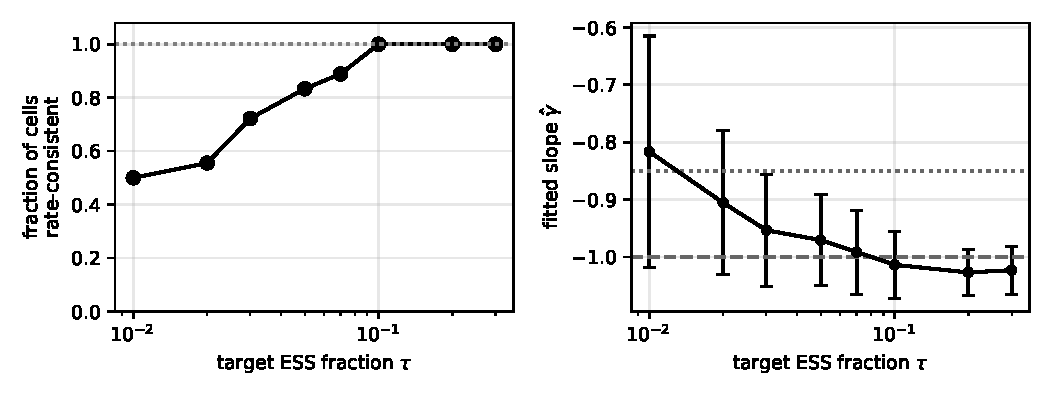
\includegraphics[width=\textwidth]{fig1.pdf}
\caption{Left: fraction of $18$ cells rate-consistent against $\tau_0$. Right: mean fitted slope with standard deviation across cells; dashed line the benchmark exponent $-1$, dotted line the tolerance $-0.85$. Data: Table~\ref{tab:boundary}.}\label{fig:boundary}
\end{figure}

\begin{figure}[h]
\centering
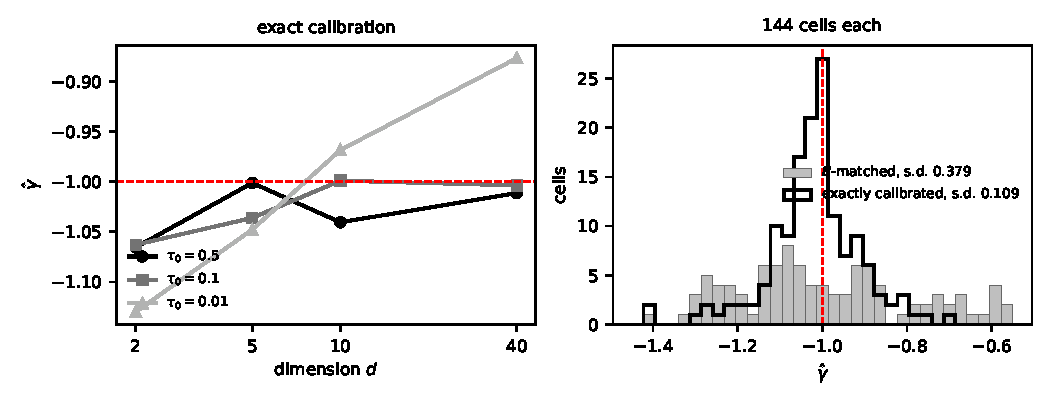
\includegraphics[width=0.48\textwidth]{fig2.pdf}\hfill
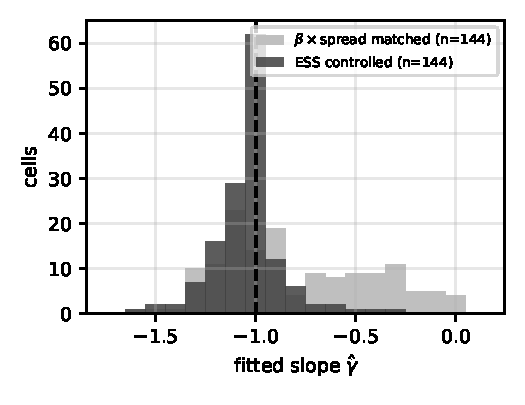
\includegraphics[width=0.48\textwidth]{fig3.pdf}
\caption{Left: fitted slope against dimension at three concentration targets under exact calibration (upper block of Table~\ref{tab:mech}); the dashed line is the benchmark exponent $-1$. Right: fitted slopes over the $144$ $B$-matched cells (s.d.\ $0.379$) against the $144$ exactly calibrated cells (s.d.\ $0.109$).}\label{fig:control}
\end{figure}

\begin{figure}[h]
\centering
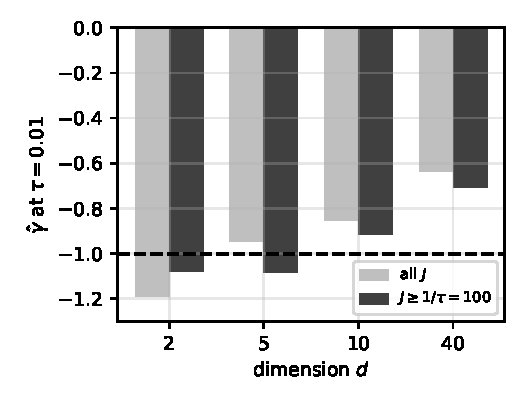
\includegraphics[width=0.48\textwidth]{fig4.pdf}\hfill
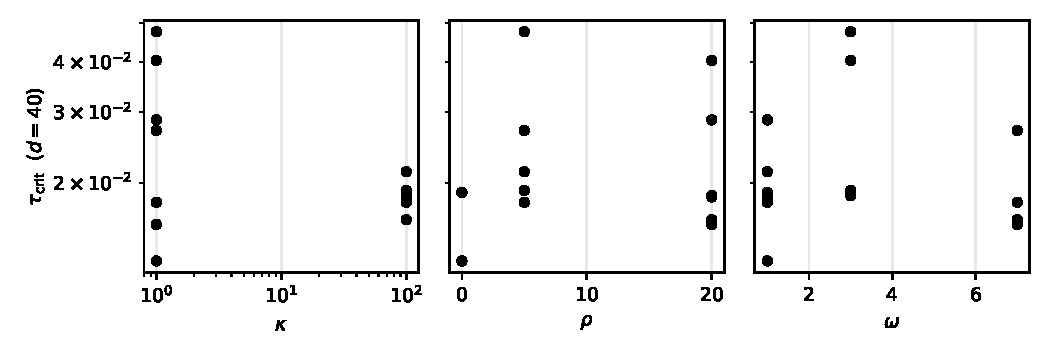
\includegraphics[width=0.48\textwidth]{fig5.pdf}
\caption{Left: magnitude of the fitted slope, $-\hat\gamma$, at $\tau_0=0.01$ by dimension, full grid and $J\ge1/\tau_0$ (Table~\ref{tab:thm}); the axis is plotted as a magnitude and every underlying slope is negative. Right: identified $\tau_{\rm crit}$ at $d=40$ against the three generating parameters of \eqref{eq:synth}; jointly $R^2=0.171$ (Section~\ref{sec:law}).}\label{fig:thm}
\end{figure}

\begin{figure}[h]
\centering
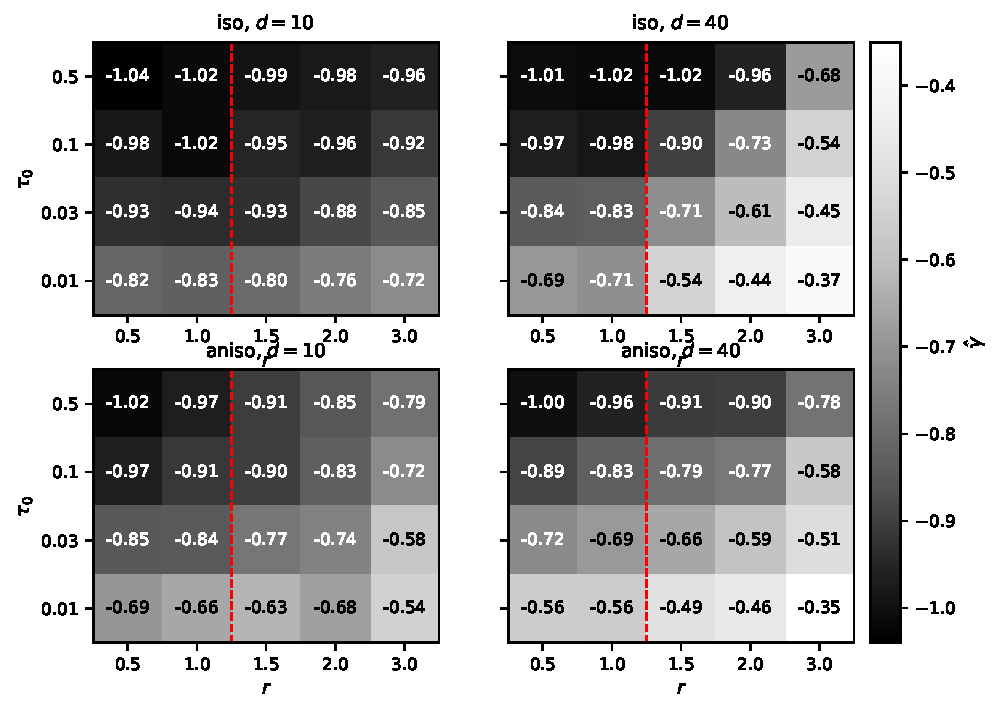
\includegraphics[width=0.92\textwidth]{fig6.pdf}
\caption{The regime map: fitted exponent over $\tau_0$ (rows, top to bottom $0.5$, $0.1$, $0.03$, $0.01$) and $r$ (columns), for both diffusion types at $d=10$ and $d=40$. The dashed vertical line is the condition boundary $r=1$. Values are the entries of Table~\ref{tab:map}, generated from the archived file rather than transcribed.}\label{fig:map}
\end{figure}

\begin{figure}[h]
\centering
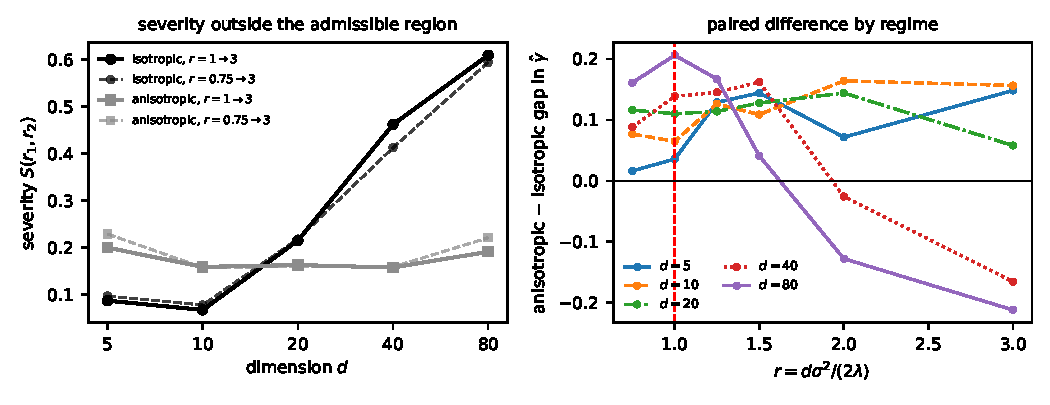
\includegraphics[width=\textwidth]{fig7.pdf}
\caption{Left: severity $S(r_1,r_2)=\hat\gamma(r_2)-\hat\gamma(r_1)$ against dimension, solid for the non-admissible contrast $S(1,3)$, which is the result relied on, and dashed for the boundary-spanning contrast $S(0.75,3)$ of Table~\ref{tab:severity}, shown as sensitivity. Positive values mean the exponent has flattened toward zero. Right: paired anisotropic-minus-isotropic gap against $r$ by dimension; the dashed vertical line is the boundary $r=1$ (Section~\ref{sec:onset}).}\label{fig:severity}
\end{figure}

\section{Results withdrawn during this work}\label{sec8}

Six results were obtained, reported internally and subsequently withdrawn after further testing: a dimension-dependent exponent $|\hat\gamma|\approx cd^{-0.57}$; a crossover ensemble size at which the rate becomes observable; an extreme-order-statistics explanation predicting exponent $2/d$; the effective sample size as a general diagnostic; the claim that concentration is the mechanism, without qualification; and three successive readings of the condition $2\lambda>d\sigma^2$, that it is inert, that it is a sharp boundary, and that degradation begins near $r=1.5$. The complete audit trail, with the evidence that produced each and the evidence that withdrew it, is in Supplementary Material~S3, and the analysis-design errors identified during the same period are in Supplementary Material~S2.

\section{Limitations}\label{sec10}

The reference ensemble is a proxy at one twentieth of the size in \cite{ghv2025}; Section~\ref{sec:refbias} finds no evidence of material bias under concentration control, but the extrapolation is noise-limited and assumes a $1/J_\infty$ form without justification. The horizon is varied only over $\{0.5,1,2\}$. The concentration-control and regime-map experiments use the centred law; Section~\ref{sec:horizon} varies it explicitly across four laws. Concentration is controlled at $t=0$ except in Section~\ref{sec:wholerun}. The modality descriptor of Section~\ref{sec:law} retains a residual correlation of $+0.58$ with frequency across the full synthetic family. Section~\ref{sec4} is upper bounds composed with upper bounds. Theorem~\ref{thm:ess} covers one of three error terms and its Chebyshev step is crude. No familywise error guarantee is claimed; Bonferroni sensitivity is reported and the out-of-condition anisotropic count in Section~\ref{sec:onset} falls from $18$ to $8$ of $75$ under it. The comparison with \cite{ghkv2025} is between a finite-run fitted exponent and a bound prefactor, which are different objects. Section~\ref{sec:onset} does not identify the mechanism of the out-of-condition degradation.

\section{Conclusions}\label{sec11}

The $r$ experiments remain target-calibrated rather than exact-calibrated, so their effect estimates may contain residual concentration confounding; only the concentration arm was rerun. The boundary $r=1$ separates the theorem-admissible from the non-admissible parameter regime, but it does not coincide with a finite-run observability threshold: admissible cells can fail the operational criterion, as three of the thirty in Section~\ref{sec:map} do, and non-admissible ones can pass it. That the two regions are different objects is the paper's central conceptual point.

One distinction governs how everything below should be read. This paper measures whether the $J^{-1}$ benchmark exponent is visible in the fitted slope of a finite run. It does not measure optimization performance, and a flat fitted exponent is not a statement that CBO optimized badly in that configuration. A method can optimize well in a regime in which no proven rate is observable, and nothing here licenses the reverse inference.


Finite-ensemble observability of the CBO mean-field rate is not determined by dimension alone. Much of the apparent dimension-dependent degradation seen under an inverse-temperature rule matched by objective spread is mediated by Boltzmann-weight concentration: with the inverse temperature solved on the reference ensemble itself, so that the achieved initial concentration equals its target exactly, controlling concentration reduces the change in fitted exponent from $d=2$ to $d=40$ from $0.96$ to $0.054$, $0.059$ and $0.078$ at the three targets, with no difference detected between any pair and no pair shown equivalent. The formal interaction between dimension and concentration is not resolved on this window, $+0.0073$ with interval $[-0.0091,+0.0227]$. Earlier versions of this experiment reported $0.030$, $0.099$ and $0.553$ under probe calibration, and $0.253$ at the tightest target under exact calibration over the full ensemble-size grid; both of those figures were products of the protocol. The tightest target cannot be realized at all below $J=100$, and four of the ten sizes in the grid sit below that bound. What remains after both corrections is small, and an audit of the nested subensembles shows that even that remainder is confounded with a dimension-dependent finite-$J$ concentration effect. A dedicated experiment controlling that concentration exactly at every ensemble size does not make the contrast vanish, but is inconclusive about the mechanism of the residual, so the remainder is reported as confounded rather than resolved. Under the declared criterion, a target $\tau_0\ge0.1$ was operationally sufficient in all $54$ cells, while the level actually required varies across cells by a factor of about seven and a half and is not predicted by the low-dimensional geometry model tested here.

A finite-sample bound for the self-normalized weighted mean makes the concentration dependence explicit as a $1/(\tau J)$ prefactor. It covers one of three error terms and does not determine the interacting-particle behaviour; the observed behaviour is consistent with the scaling.

A joint sweep of concentration against the parameter-condition ratio moves the exponent on both axes in three of four panels, and leaves their interaction unresolved: the pre-specified rule required three of four interval exclusions with a consistent sign and one was obtained. Beyond the parameter condition, the onset location cannot be distinguished from $r=1$ on any grid we ran, and that experiment is not powered to locate it; the severity is the result that is resolved, growing at $+0.144$ per doubling of dimension for isotropic diffusion on the non-admissible contrast, interval $[+0.123,+0.164]$, while no systematic dimension trend was detected for anisotropic diffusion over the tested dimensions, $-0.002$ with interval $[-0.030,+0.027]$. Paired on shared realizations the two types change sign between $r=1.5$ and $r=2$ at $d=40$ and $d=80$, with the standing caveat that the energy matching holds nominally and not in realized trajectories once $r\ge2$.

Some published CBO demonstrations use very large fixed inverse temperatures --- $\alpha=10^{15}$ in the two numerical illustrations of \cite{fkr2024}, the Rastrigin experiment in dimension two with $N=32\,000$ agents, $\lambda=1$, $\sigma=0.1$, $\Delta t=0.01$, and the one-dimensional variance comparison with $N=320\,000$ and $\sigma=0.5$ --- at which the weights can become numerically saturated, in which case the consensus point is effectively the arg min. Corollary~\ref{cor:notartifact} shows the underlying weight concentration is not an artefact of the floating-point format. It is also the regime in which we can measure no proven rate at all.

\backmatter

\begin{appendices}
\section{Supplementary Material}\label{appA}
Three blocks of supporting material are provided as Supplementary Information rather than in the main text, because none of them is required to follow the experimental argument and each carries a large surface of technical detail: (i) the worst-case tracing of the mean-field constant chain of \cite{fkr2024}, including the objective-dependent branch and the refinement of the informal lower bound on $\alpha_0$; (ii) the complete log of analysis-design errors identified and corrected during this work, with the consequence and the fix for each; and (iii) the detailed record of the six withdrawn results. Section~\ref{sec8} retains a short summary of the withdrawn results, and the falsification record is referred to at the points in the text where it is relevant.
\end{appendices}

\bmhead{Supplementary information}
All scripts are single-file and depend only on NumPy. Each pre-specified criterion is stated in the docstring of the script that applies it and is present in the archived copy of that script, which is the version executed; the criteria for the regime map of Section~\ref{sec:map} were fixed in \texttt{regimemap.py} before any cell of that design had been run. Per-realization CSV files are archived for every confirmatory run in Table~\ref{tab:matrix}. For the two exploratory rows marked $\dagger$ the generating script, the aggregate outputs and the console log are archived but the original per-realization CSV was lost to an output overwrite; both rows belong to withdrawn results and no claim in Sections~\ref{sec:mech} onward rests on either. Console output with the manuscript, together with a reanalysis script that recomputes the noise floor, the fitting-window sensitivity, the equivalence tests, the change-point intervals and the tolerance and Bonferroni tables from the archived files. Each script prints its parameters, seeds, Python and NumPy versions and platform at execution.

\bmhead{Acknowledgements}
The author thanks colleagues for constructive feedback on earlier versions, which corrected an incorrect inequality in what is now Lemma~\ref{lem:sat}, an overstatement of the sufficiency claim, an invalid impossibility inference in Section~\ref{sec:law}, an incorrect asymptotic direction in Section~\ref{sec4}, an incomplete lower-growth argument for Rosenbrock now completed in Proposition~\ref{prop:rosen}, and the absence of equivalence testing and change-point analysis in Sections~\ref{sec:aniso} and \ref{sec:onset}.

\section*{Declarations}
\begin{itemize}
\item Funding: none.
\item Competing interests: the author declares none.
\item Data availability: scripts and result files are deposited at \url{https://doi.org/10.5281/zenodo.22068685}, with one exception. The per-realization files for the two exploratory rows marked $\dagger$ in Table~\ref{tab:matrix} were lost to an output overwrite; for those rows the generating script, the aggregate outputs and the console log are archived. Both rows belong to withdrawn results and no reported conclusion rests on them.
\end{itemize}

\begin{thebibliography}{99}

\bibitem{pinnau2017}
Pinnau, R., Totzeck, C., Tse, O., Martin, S.: A consensus-based model for global optimization and its mean-field limit. Math. Models Methods Appl. Sci. \textbf{27}(1), 183--204 (2017). \url{https://doi.org/10.1142/S0218202517400061}

\bibitem{carrillo2018}
Carrillo, J.A., Choi, Y.-P., Totzeck, C., Tse, O.: An analytical framework for consensus-based global optimization method. Math. Models Methods Appl. Sci. \textbf{28}(6), 1037--1066 (2018). \url{https://doi.org/10.1142/S0218202518500276}

\bibitem{fkr2024}
Fornasier, M., Klock, T., Riedl, K.: Consensus-based optimization methods converge globally. SIAM J. Optim. \textbf{34}(3), 2973--3004 (2024). \url{https://doi.org/10.1137/22M1527805}. Also available as arXiv:2103.15130. Every result of this paper cited here is referred to by its theorem, lemma, proposition or remark number, which is common to both versions; no bare equation number is used. The parameters of the two numerical illustrations quoted in Section~\ref{sec5} are described by content rather than by figure number, so that they can be located in either version

\bibitem{ghv2025}
Gerber, N.J., Hoffmann, F., Vaes, U.: Mean-field limits for consensus-based optimization and sampling. ESAIM Control Optim. Calc. Var. \textbf{31}, Paper No. 74 (2025). \url{https://doi.org/10.1051/cocv/2025060}. Also available as arXiv:2312.07373

\bibitem{ghkv2025}
Gerber, N., Hoffmann, F., Kim, D., Vaes, U.: Uniform-in-time propagation of chaos for consensus-based optimization. arXiv preprint arXiv:2505.08669 (2025)

\bibitem{hk2025}
Huang, H., Kouhkouh, H.: Uniform-in-time mean-field limit estimate for the consensus-based optimization. ESAIM Control Optim. Calc. Var. \textbf{31}, Paper No. 69 (2025)

\bibitem{bez2026}
Bayraktar, E., Ekren, I., Zhou, H.: Uniform-in-time weak propagation of chaos for consensus-based optimization. Ann. Appl. Probab. \textbf{36}(3), 2387--2426 (2026). \url{https://doi.org/10.1214/25-AAP2281}. The result is stated on a bounded search domain

\bibitem{kwz2024}
Ko\ss{}, M., Weissmann, S., Zech, J.: On the mean-field limit of consensus-based methods. Math. Methods Appl. Sci. \textbf{49}, 4214--4240 (2026). \url{https://doi.org/10.1002/mma.70343}

\bibitem{beddrich2024}
Beddrich, J., Chenchene, E., Fornasier, M., Huang, H., Wohlmuth, B.: Constrained consensus-based optimization and numerical heuristics for the few particle regime. J. Global Optim. (2026). \url{https://doi.org/10.1007/s10898-026-01612-x}

\bibitem{fhps2020}
Fornasier, M., Huang, H., Pareschi, L., S\"unnen, P.: Consensus-based optimization on hypersurfaces: well-posedness and mean-field limit. Math. Models Methods Appl. Sci. \textbf{30}(14), 2725--2751 (2020)

\bibitem{huangqiu2022}
Huang, H., Qiu, J.: On the mean-field limit for the consensus-based optimization. Math. Methods Appl. Sci. \textbf{45}(12), 7814--7831 (2022)

\bibitem{borghi2023}
Borghi, G., Herty, M., Pareschi, L.: Constrained consensus-based optimization. SIAM J. Optim. \textbf{33}(1), 211--236 (2023)

\bibitem{carrillo2021}
Carrillo, J.A., Jin, S., Li, L., Zhu, Y.: A consensus-based global optimization method for high dimensional machine learning problems. ESAIM Control Optim. Calc. Var. \textbf{27}(suppl.), Paper No. S5 (2021)

\bibitem{agapiou2017}
Agapiou, S., Papaspiliopoulos, O., Sanz-Alonso, D., Stuart, A.M.: Importance sampling: intrinsic dimension and computational cost. Statist. Sci. \textbf{32}(3), 405--431 (2017). \url{https://doi.org/10.1214/17-STS611}

\bibitem{doukhan2009}
Doukhan, P., Lang, G.: Evaluation for moments of a ratio with application to regression estimation. Bernoulli \textbf{15}(4), 1259--1286 (2009). \url{https://doi.org/10.3150/09-BEJ190}

\bibitem{frrs2025}
Fornasier, M., Richt\'arik, P., Riedl, K., Sun, L.: Consensus-based optimisation with truncated noise. European J. Appl. Math. \textbf{36}(2), 292--315 (2025). \url{https://doi.org/10.1017/S095679252400007X}

\bibitem{cbx2024}
Bailo, R., Barbaro, A., Gomes, S.N., Riedl, K., Roith, T., Totzeck, C., Vaes, U.: CBX: Python and Julia packages for consensus-based interacting particle methods. J. Open Source Softw. \textbf{9}(98), 6611 (2024). \url{https://doi.org/10.21105/joss.06611}

\end{thebibliography}

\end{document}
